\documentclass{article}
\usepackage{graphicx}
\graphicspath{{figures/}}
\usepackage{amsmath}
\usepackage{booktabs}
\usepackage{float}
\usepackage{natbib}
\usepackage{microtype}
\setlength{\emergencystretch}{3em}

\title{Equal Accuracy, Unequal Cost: \\ Channel Dependence in PatchTST under Controlled Coupling}
\author{Adi Mendelowitz}
\date{June 2026}

\begin{document}

    \maketitle

    \begin{abstract}
        Channel-independent (CI) and channel-dependent (CD) variants of PatchTST are typically compared on observational
        benchmarks where correlation strength, dimensionality, and temporal dynamics all vary at once, leaving no clean way to
        attribute either variant win to any single cause. We isolate one factor at a time. A factorial AR(1) experiment varies
        contemporaneous correlation $\rho$ and variate count $C$ while Granger non-causality holds across channels by
        construction, and a leader-follower VAR(1) experiment introduces lag-1 coupling of controllable strength $\gamma$. On
        the synthetic grid we detect no consistent CD advantage at the $1\%$ level: the grand-mean CD$-$CI difference is
        $+0.0013$ MSE (95\% CI $[-0.0002, +0.0028]$) over five seeds, with a pooled within-cell detection half-width of 0.0063
        MSE, so any global CD gain (averaged across the nine AR(1) cells) above roughly $0.63\%$ of the CI mean would have moved
        the interval off zero, and none did. Under the original early-stopping protocol an apparent CD deficit emerges under
        lagged coupling and grows with $\gamma$, though it stays inside our $1\%$ band throughout. An instrumented diagnostic at
        the leader-follower $\gamma=0.6$ cell documents a mechanism without explaining the deficit: CD reaches a sharper,
        earlier validation minimum than CI and degrades past it, but the protocol already restores validation-best weights, so
        the gap is not a selection artefact. Fresh reruns of that cell give CD$-$CI of $-0.0019$ MSE (95\% CI
        $[-0.0105, +0.0066]$) against the original $+0.0079$, a run-to-run spread comparable to the effect itself at five seeds.
        A closed-form analysis of the generative model shows this near-parity is analytically expected, not merely observed: at
        the evaluation horizon, no predictor, channel-independent or channel-dependent, has any cross-channel signal left to
        exploit. A cross-variate prediction head ties CI at every $\gamma$ and removes the coupling-dependent widening, locating
        that widening in the shared head rather than the encoder. Matching the gradient-update budget across modes removes the
        deficit, which rules out the per-epoch step-count asymmetry as its source, and a block-covariance family carries the same
        no-advantage finding beyond compound-symmetry correlation. Across every tested synthetic cell (AR(1), leader-follower,
        and block-covariance) the absolute CD$-$CI difference stays inside a pre-specified $1\%$ relative-MSE band in both
        directions. What does not equalise is cost: CD requires smaller feasible batches and far more gradient steps per epoch,
        its batch size collapses to one at $C=84$ in the main grid, and at $C=321$ (ECL) a CD epoch costs roughly 956\,s at
        batch 8; in a single-seed comparison at $H \in \{96, 336\}$, CD trails CI by 5.6--7.6\%. On the observational ETTh1 ($C=7$), a matched-budget comparison still gives CI
        a modest but reliable edge (pooled CD$-$CI of $+0.0147$ MSE, 95\% CI $[+0.0047, +0.0246]$, significant at horizons 96
        and 720). CI is the better default on accuracy per unit compute. All findings are scoped to PatchTST's flattened-token CD formulation, the
        generative families studied, and a single-T4 training budget.

    \end{abstract}


    \section{Introduction}
    \label{sec:intro}

    Whether channel-independent (CI) or channel-dependent (CD) architectures forecast better has been judged almost entirely
    on observational benchmarks, where many properties of the data move together across datasets. Such a win identifies
    which model is stronger on those particular series, but not why. Here we control the generative process: synthetic AR(1) and
    leader-follower VAR(1) families that vary instantaneous correlation, lagged cross-channel dependence, and variate count
    independently, with ETTh1 and ECL as real-data context rather than primary evidence.

    The first experiment generates data from an AR(1) process with diagonal transition and compound-symmetry covariance, so
    the only cross-channel structure is instantaneous correlation. The second introduces lagged coupling through a
    leader-follower VAR(1) process where coupling strength $\gamma$ is a controllable parameter. No point in the tested
    coupling-structure space yielded a consistent CD advantage. Section~\ref{sec:setup} describes the experimental design,
    Section~\ref{sec:results} presents the AR(1) grid and real-data results, Section~\ref{sec:analysis} covers the
    leader-follower experiments, Section~\ref{sec:robustness} presents the fair-protocol robustness controls, and the
    remaining sections discuss limitations, related work, and conclusions.

    \subsection{Research Questions and Scope}

    CI architectures like PatchTST have become strong baselines for multivariate time series forecasting despite ignoring
    cross-channel interactions in their attention layers~\citep{nie2023patchtst}. At the same time, iTransformer, LIFT, and
    Abdelmalak et al.\ each report settings where modelling channel dependence explicitly yields clear
    gains~\citep{liu2024itransformer,zhao2024rethinkingchanneldependence,%
        abdelmalak2025channeldependence}. None of these results are directly comparable: the architectures, datasets,
    and notions of cross-channel structure all differ across papers. There is no account of which
    property of the data tips the balance.

    We focus on one specific part of that question: multivariate processes in which channels share \emph{instantaneous}
    correlation but have no lagged cross-channel dependence in the dynamics. Concretely, we use a vector AR(1) process with
    a diagonal transition matrix and compound-symmetry covariance, where $\rho$ controls contemporaneous correlation while
    Granger non-causality holds across all channel pairs by construction. Two questions frame the work:

    \begin{quote}
        \textbf{RQ1.} In a setting where channels share purely instantaneous correlation, even at high $\rho$ and high
        dimensionality, and no lagged cross-channel dependence exists by construction, does a channel-dependent PatchTST variant
        achieve meaningfully better forecast accuracy than its channel-independent counterpart?
    \end{quote}

    \begin{quote}
        \textbf{RQ2.} When lagged cross-channel coupling is introduced at controlled strength $\gamma$ via a leader-follower
        VAR(1) process, does CD outperform CI consistently as $\gamma$ grows, and does this depend on the patch resolution used?
    \end{quote}

    RQ1 is answered by a $C \times \rho \times \text{mode}$ factorial experiment on AR(1) data where Granger non-causality
    holds by construction. RQ2 is answered by two companion experiments: a $\gamma$ sweep at fixed patch size $P = 16$, and
    a joint sweep over $\gamma \in \{0.0, 0.3, 0.6, 0.9\}$ and $P \in \{2, 4, 8, 16\}$ testing whether finer patch
    resolution concentrates lag-1 coupling within individual patches and thereby gives CD's attention a detectable signal.
    That second sweep does not cover its full grid. CD trains at $P \in \{4, 8, 16\}$; at $P = 2$ the flattened CD sequence
    reaches $21 \times 511 = 10{,}731$ tokens and exceeds T4 memory at any batch size, so the finest resolution, the one
    where a lag-1 relation falls across adjacent patches rather than inside a single patch, carries CI runs only. RQ2 is
    therefore answered over $P \in \{4, 8, 16\}$ and left open at $P = 2$.

    Within the regimes actually tested, both RQ1 and RQ2 come back null at our $1\%$ practical threshold: small differences
    exist, but none clears the bar. Section~\ref{sec:theoretical_bound} establishes that this null is what the generative
    model predicts rather than only what the training runs produced: at the evaluation horizon $h = 96$, the analytical gap
    between a full-information and a channel-restricted predictor has closed to zero width for every tested $\gamma$, so no
    predictor of either kind has cross-channel signal left to exploit. The comparison at $h = 96$ therefore cannot
    discriminate the architectures even in principle, and RQ2's null is scoped to that horizon; the short-horizon regime,
    where the ceilings separate, is left open and named in the Limitations. A set of fair-protocol controls
    (Section~\ref{sec:robustness}) then shows that the apparent CD deficit under lagged coupling does not survive a matched
    update budget or a cross-variate head, and that it is small relative to run-to-run variation at five seeds.

    Our conclusions are scoped accordingly: we make no broad claim that CD is unnecessary. We show that purely instantaneous
    correlation, regardless of strength or variate count, is not sufficient for CD to gain an advantage over CI under
    PatchTST's architecture, and that this null result extends to lag-1 coupling at the strengths tested and at patch
    resolutions $P \in \{4, 8, 16\}$.


    \section{Experimental Setup}
    \label{sec:setup}

    \subsection{Synthetic Data}

    We generate multivariate time series from a vector AR(1) process:
    \begin{equation}
        x_{t} = \phi\, x_{t-1} + \epsilon_{t}, \qquad \epsilon_{t} \sim \mathcal{N}(0,\,\Sigma),
    \end{equation}
    where $\phi = 0.8$ and $\Sigma$ has compound-symmetry structure: $\Sigma_{ii} = 1$ and $\Sigma_{ij} = \rho$ for
    $i \neq j$. The parameter $\rho$ directly controls pairwise contemporaneous correlation while the transition matrix
    remains diagonal. We discard 1000 burn-in steps before recording observations.

    For each configuration in this grid we generate 14,400 timesteps (13,400 for seeds $\{42, 123, 456\}$;
    Table~\ref{tab:synth_protocols}) and split them 60/20/20 into train, validation, and test sets; the table also gives
    the corresponding figures for the other synthetic families. All
    splits are normalised with per-channel z-score statistics fit on the training set only. We vary three factors
    independently: number of channels $C \in \{7, 21, 84\}$, correlation strength $\rho \in \{0.1, 0.5, 0.9\}$, and model
    mode $\in \{\text{CI}, \text{CD}, \text{DLinear}\}$, with five random seeds $\{42, 123, 456, 789, 1011\}$ per cell, yielding 135
    runs in total. We report the empirical pairwise Pearson correlation of the training data alongside the nominal $\rho$ to
    confirm intended data-generating process behaviour.

    The synthetic families in this paper do not all share one generator. The AR(1) grid, the block-covariance family, and
    the leader-follower $\gamma$-sweep use the process specified above, differing only in the innovation covariance, the
    transition matrix, and (within the AR(1) grid) the series length, which takes two values across its five seeds; the $(P, \gamma)$ boundary sweep
    of Section~\ref{sec:analysis} uses a separate generator with iid innovations, a longer series, and a different split.
    Table~\ref{tab:synth_protocols} states each family's protocol explicitly. One consequence is worth stating plainly:
    because the boundary protocol differs in innovation covariance, series length, and split simultaneously, absolute MSE
    levels are not comparable between it and the other three families, and we do not compare them. Within each family the
    CD/CI ratio is computed against a CI arm trained under that same protocol, so the ratio remains the comparable
    quantity throughout.

    \begin{table}[H]
        \centering
        \caption{Data-generating protocols for the four synthetic families. All are VAR(1) at $\phi = 0.8$, use $L = 512$
            and $H = 96$, and normalise by per-channel z-score statistics fit on the training split only. Three share
            a single protocol and differ only in covariance and transition structure; the boundary sweep differs in
            several further respects. Innovation scale ($\sigma = 0.1$ versus unit) is removed by z-scoring, and the
            absence of burn-in is immaterial at $\phi = 0.8$ over 20{,}000 steps; neither is treated as a substantive
            difference. The substantive ones are the innovation covariance, the series length, and the split. The
            boundary family's recorded $\rho = 0.5$ is a schema constant carried for mergeability, not a property of
            its data: its innovations are iid, so no contemporaneous cross-channel correlation is present.}
        \label{tab:synth_protocols}
        \begin{tabular}{lcccc}
            \toprule
            & AR(1) grid             & Block-cov.                  & Leader-follower                          & Boundary                               \\
            & (Sec.~\ref{sec:setup}) & (Sec.~\ref{sec:robustness}) & $\gamma$-sweep (Sec.~\ref{sec:analysis}) & $(P,\gamma)$ (Sec.~\ref{sec:analysis}) \\
            \midrule
            Transition matrix      & $\phi\mathbf{I}$       & $\phi\mathbf{I}$            & $A(\gamma)$ lower-tri                    & $A(\gamma)$ lower-tri                  \\
            Innovation cov.        & comp.\ sym.\ $\rho$    & block $\rho_{\text{in}}$, 0 & comp.\ sym.\ $\rho = 0.5$ & iid (diagonal) \\
            Innovation scale       & unit                   & unit                        & unit                                     & $\sigma = 0.1$                         \\
            Burn-in steps          & 1000                   & 1000                        & 1000                                     & none                                   \\
            Timesteps $T$$^{c}$    & 13{,}400 / 14{,}400    & 14{,}400                    & 14{,}400                                 & 20{,}000                               \\
            Split                  & 60/20/20\,\%           & 60/20/20\,\%                & 60/20/20\,\%                             & 70/10/20\,\%                           \\
            Train windows$^{a,c}$  & 7{,}433 / 8{,}033      & 8{,}033                     & 8{,}033                                  & 13{,}393                               \\
            Partial final batch    & kept                   & kept                        & kept                                     & dropped                                \\
            Channels $C$           & $\{7, 21, 84\}$        & $\{21, 84\}$                & 21                                       & 21                                     \\
            Coupling $\gamma$      & ---                    & ---                         & $\{0, .3, .6, .9\}$                      & $\{0, .3, .6, .9\}$                    \\
            Patch $P$ / stride $S$ & 16 / 8                 & 16 / 8                      & 16 / 8                                   & $P$ / $P/2$, $P \in \{2,4,8,16\}$      \\
            Modes$^{b}$            & CI, CD, DLinear        & CI, CD, DLinear             & CI, CD, DLinear                          & CI, CD                                 \\
            \bottomrule
        \end{tabular}

        \vspace{0.5em}
        {\footnotesize
            $^{a}$ Training windows $= \lfloor T \cdot f_{\text{train}} \rfloor - L - H + 1$ at $L = 512$, $H = 96$.\\
            $^{b}$ Modes attempted. Which cells completed under compute constraints is stated per experiment.\\
            $^{c}$ AR(1) grid only: seeds $\{42, 123, 456\}$ were generated with 13{,}400 usable timesteps and seeds
            $\{789, 1011\}$ with 14{,}400, giving 7{,}433 and 8{,}033 training windows respectively. Per-seed CD$-$CI
        differences are unaffected, since both modes of a given seed share that seed's series; grid means in
        Table~\ref{tab:synthetic} average over both. Table~\ref{tab:batch_sizes} reports the 7{,}433 figures.}
    \end{table}


    \textbf{Dynamical structure.} Because the transition operator $\phi\mathbf{I}$ is diagonal, each variate's next value
    depends only on its own past. Granger non-causality holds exactly across all channel pairs: all cross-variate dependence
    arises from the contemporaneous covariance $\Sigma$, not from the dynamics. The transition matrix
    $A^k = (\phi\mathbf{I})^k = \phi^k \mathbf{I}$ has zero off-diagonal entries at every power, so no channel's past
    dynamically informs another channel's future: there are no cross-channel dynamical coefficients. This does not mean
    lagged cross-covariance between $\Sigma$-correlated channels is exactly zero at every $k$, but that no such covariance,
    were it present, would carry Granger-predictive information beyond what each channel's own history already gives.
    Contemporaneous correlation in $\Sigma$ does not provide a predictive signal
    because innovations are unobserved at prediction time. The leader-follower experiments in Section~\ref{sec:analysis}
    introduce the complementary case where the transition operator structurally links one variate's future to another's past.

    \textbf{Covariance design.} Compound-symmetry assigns the same pairwise correlation $\rho$ to every channel pair, giving
    CD no differential block structure or correlation hierarchy to exploit. This is the configuration most hostile to CD
    under instantaneous-only coupling: if CD cannot gain an advantage here, contemporaneous correlation alone will not be
    sufficient at any other covariance structure within this family.

    \textbf{Prediction horizon.} All synthetic AR(1) runs use $\text{pred\_len} = 96$, matching the shortest horizon in the
    ETTh1 experiments.

    \subsection{Real-World Datasets}

    \textbf{ETTh1.} Hourly measurements of 7 variates (oil temperature and six power-load features) from a Chinese
    electrical transformer. We use the standard train/val/test split of 8640/2880/2880 timesteps. The mean absolute
    off-diagonal Pearson correlation at lag~0 across the training split is 0.311 (median 0.233), indicating moderate
    contemporaneous cross-variate correlation.

    \textbf{ECL (Electricity Consuming Load).} Hourly electricity consumption for 321 clients over 26,304 timesteps. (The
    iTransformer paper~\citep{liu2024itransformer} reports 26,352 rows; the difference reflects a minor dataset version
    discrepancy and does not affect the experimental protocol.) We apply proportional 60/20/20 splitting following Liu et
    al., yielding 15,813 train / 5,247 validation / 5,244 test rows. The mean absolute off-diagonal Pearson correlation at
    lag~0 is 0.503 (median 0.483), substantially higher than ETTh1. All data are normalised with per-channel z-score
    statistics fit on the training set only.

    \subsection{Models}

    PatchTST is the backbone for both CI and CD modes because the two modes differ in exactly one thing: whether
    self-attention operates within each variate's patch sequence independently or across all variates' patch sequences
    jointly. Patch extraction, linear projection, Transformer encoder, training procedure, and hyperparameters are otherwise
    shared, making this the most direct available test of the CD/CI distinction without entangling it with other
    architectural choices. iTransformer would confound the comparison with its inverted embedding design; Crossformer with
    its two-stage routing attention. All findings are conditioned on PatchTST's patch-based representation and the lookback
    window and patch granularity used.

    We implement PatchTST~\citep{nie2023patchtst} from scratch in PyTorch, supporting both modes.

    \textbf{Channel-Independent (CI).} Each variate is processed separately. An input of shape $(B, L, C)$ is reshaped to
    $(B \cdot C, L)$, split into patches of length $P$ with stride $S$, and passed through a shared Transformer encoder.
    The encoder sees $N$ patches per variate.

    \textbf{Channel-Dependent (CD).} All variates are processed jointly. After patching, tokens from all variates are
    concatenated along the sequence dimension before the encoder, giving an input of shape $(B,\, C \cdot N,\, D)$.
    Self-attention operates over all $C \cdot N$ tokens simultaneously, allowing the model to attend across variates. After
    encoding, the output is split back into $C$ per-variate representations before a shared linear head projects each
    variate to the prediction horizon. The encoder mixes cross-variate information; the head does not. Tokens carry no
    explicit channel-identity or temporal-position embedding; both are encoded solely through fixed ordering,
    channel-major for CD (all $N$ patches of channel 0, then channel 1, and so on) and the natural patch sequence for CI.
    This holds for every CD result reported in this paper.

    For the synthetic experiments and ETTh1 we use $L = 512$, $P = 16$, $S = 8$, giving
    \begin{equation}
        N = \left\lfloor \frac{L - P}{S} \right\rfloor + 1
        = \left\lfloor \frac{512 - 16}{8} \right\rfloor + 1 = 63
    \end{equation}
    patches per variate. For ECL we use $L = 96$ following iTransformer~\citep{liu2024itransformer}, giving $N = 11$ patches
    per variate and $C \cdot N = 321 \times 11 = 3531$ tokens for CD. All remaining architectural hyperparameters are listed
    in Table~\ref{tab:arch}.

    \begin{table}[H]
        \centering
        \caption{Architectural hyperparameters. Synthetic and ETTh1 share one configuration;
        ECL uses a wider model to accommodate 321 variates.}
        \label{tab:arch}
        \begin{tabular}{lcc}
            \toprule
            Hyperparameter          & Synthetic + ETTh1 & ECL \\
            \midrule
            $d_{\text{model}}$      & 64                & 128 \\
            Attention heads         & 8                 & 16  \\
            Encoder layers          & 3                 & 3   \\
            Dropout                 & 0.2               & 0.2 \\
            Sequence length $L$     & 512               & 96  \\
            Patch size $P$          & 16                & 16  \\
            Stride $S$              & 8                 & 8   \\
            Patches per variate $N$ & 63                & 11  \\
            \bottomrule
        \end{tabular}
    \end{table}

    We include DLinear~\citep{zeng2023transformerseffectivetimeseries} as a linear baseline. DLinear decomposes each
    variate's lookback window into trend (moving-average filter with kernel size 25) and remainder, then applies separate
    channel-independent linear maps from $L$ to $H$ for each component, summing the two outputs. It is the most competitive
    non-Transformer baseline on standard benchmarks and sets a natural lower bar for what qualifies as learned temporal
    structure. The DLinear values in Tables~\ref{tab:synthetic} and~\ref{tab:lf_p16} are produced by a dedicated
    re-run using this full decomposition; CI and CD values in Table~\ref{tab:lf_p16} are from a separate set of runs
    using the same windowing and seeds.

    \subsection{Training Regime}

    PatchTST (CI and CD) is trained with AdamW ($\text{lr} = 10^{-4}$, $\text{weight\_decay} = 10^{-4}$), a cosine
    learning-rate schedule with linear warm-up, gradient clipping at $\text{max\_norm} = 1.0$, and FP16 mixed precision
    (autocast + GradScaler). DLinear uses the same optimiser without warm-up. Early stopping is applied on validation MSE
    with patience 10 and a maximum of 100 epochs for ETTh1 and 50 epochs for all other experiments; the validation-best
    checkpoint is restored and evaluated in every case. All experiments run on a single NVIDIA T4 16\,GB GPU.

    \textbf{Batch sizes.} T4 memory constraints force different batch sizes between CI and CD at large $C$, creating an
    asymmetry in per-epoch gradient update counts. Table~\ref{tab:batch_sizes} reports these counts for each configuration.

    \begin{table}[H]
        \centering
        \caption{Batch sizes and gradient update counts per epoch by mode and $C$. The Ratio column is CD steps / CI
        steps. At $C=84$, steps/epoch reflects the 7,433-window figure (seeds $\{42, 123, 456\}$); seeds $\{789, 1011\}$ used
        a longer series (8,033 windows, Table~\ref{tab:synth_protocols}), so their per-epoch step counts differ proportionally,
        though CD/CI ratios are unaffected since both modes of a given seed share that seed's window count.}
        \label{tab:batch_sizes}
        \begin{tabular}{cccccr}
            \toprule
            $C$ & CI batch & CD batch & CI steps/epoch & CD steps/epoch & Ratio        \\
            \midrule
            7   & 128      & 64       & 59             & 117            & $2.0\times$  \\
            21  & 128      & 8        & 59             & 930            & $15.8\times$ \\
            84  & 32       & 1        & 233            & 7433           & $31.9\times$ \\
            \bottomrule
        \end{tabular}
    \end{table}

    For ETTh1 both modes use batch size 32 under the matched-budget protocol below. For ECL both modes use batch size 8
    (1,953 steps per epoch at $H = 96$; 1,923 at $H = 336$).

    \textbf{Step-count confound.} At $C = 84$, CD runs with batch size 1, giving $31.9\times$ more gradient updates per
    epoch than CI. The cause is a hardware memory limit, not a deliberate experimental choice. We log \texttt{total\_steps} for every run and
    report it alongside results. The significance of this asymmetry for interpreting the null result is discussed in
    Section~\ref{sec:results}.

    \textbf{Matched-budget ETTh1 protocol.} Both CI and CD use batch size 32, $\text{warmup\_epochs} = 10$, and a
    minimum of 15 epochs before early stopping may fire. The identical batch size gives both modes the same number of
    gradient updates per epoch at every horizon (252, 249, 244, and 232 at $H \in \{96, 192, 336, 720\}$ respectively),
    removing the step-count confound present in earlier runs. The minimum-epoch floor prevents a degenerate epoch-one stop
    without inflating test MSE, since the best validation checkpoint is still used for evaluation.

    \textbf{ECL CD cost.} At $C = 321$ and $L = 96$ the flattened CD sequence is 3{,}531 tokens, and a CD training epoch
    takes roughly 956\,s on the T4 at batch 8 (measured at $H = 336$), against roughly 108\,s for a CI epoch at the same
horizon and batch size -- an $8.9\times$ cost ratio -- so a worst-case 50-epoch run would exceed a single
    12-hour session on wall-clock time. Early stopping resolves this in practice: the completed CD runs stopped at epochs
    23 ($H = 96$) and 17 ($H = 336$), the latter costing about 4.5 GPU-hours, and per-epoch checkpointing with
    cross-session resumption covers the worst case. Throughout this paper, \emph{commodity GPU budget} refers to
    single-T4 training with a 12-hour wall-clock limit, as in a standard Kaggle notebook session. Kaggle's dual-T4 accelerator
    option was selected for these sessions, but all training and inference reported here remains single-device: no run uses
    more than one GPU through model or data parallelism, so the reported wall-clock figures reflect one T4's actual
    utilisation throughout.


    \section{Results}
    \label{sec:results}

    \subsection{Synthetic AR(1) Grid}

    Table~\ref{tab:synthetic} shows mean test MSE over five seeds for each cell. CI and CD track each other almost
    exactly across the grid. The largest mean difference is 0.0054 MSE units at $C = 84$, $\rho = 0.9$, and the
    direction of the difference is not consistent across the grid: CI leads at $C = 7$ across all $\rho$, at $C = 21$
    for $\rho \in \{0.1, 0.5\}$, and at $C = 84$ for $\rho \in \{0.5, 0.9\}$; CD leads marginally at $C = 21$, $\rho = 0.9$ and at $C = 84$, $\rho = 0.1$. At $C \in \{21, 84\}$
    DLinear is consistently worse than both PatchTST variants, confirming that the Transformer representations add value
    once dimensionality increases. At $C = 7$, DLinear is within roughly $1\%$ of the PatchTST variants across $\rho$ and
    occasionally slightly better; the CD/CI comparison remains the central question and both variants behave identically
    regardless of the DLinear baseline's position.

    \begin{table}[H]
        \centering
        \caption{Mean test MSE over seeds $\{42, 123, 456, 789, 1011\}$ for the synthetic AR(1) grid.
        CD/CI above 1.0 favours CI; below 1.0 favours CD.}
        \label{tab:synthetic}
        \begin{tabular}{ccrrrr}
            \toprule
            $C$ & $\rho$ & CI     & CD     & DLinear & CD/CI  \\
            \midrule
            7   & 0.1    & 1.0282 & 1.0298 & 1.0404  & 1.0016 \\
            7   & 0.5    & 1.0404 & 1.0412 & 1.0557  & 1.0008 \\
            7   & 0.9    & 1.0642 & 1.0653 & 1.1064  & 1.0011 \\
            \midrule
            21  & 0.1    & 0.9931 & 0.9950 & 1.0013  & 1.0019 \\
            21  & 0.5    & 1.0179 & 1.0189 & 1.0339  & 1.0010 \\
            21  & 0.9    & 1.0327 & 1.0311 & 1.0595  & 0.9984 \\
            \midrule
            84  & 0.1    & 0.9832 & 0.9831 & 0.9831  & 0.9999 \\
            84  & 0.5    & 0.9752 & 0.9764 & 0.9781  & 1.0012 \\
            84  & 0.9    & 0.9759 & 0.9813 & 0.9942  & 1.0056 \\
            \bottomrule
        \end{tabular}
    \end{table}

    \begin{figure}[H]
        \centering
        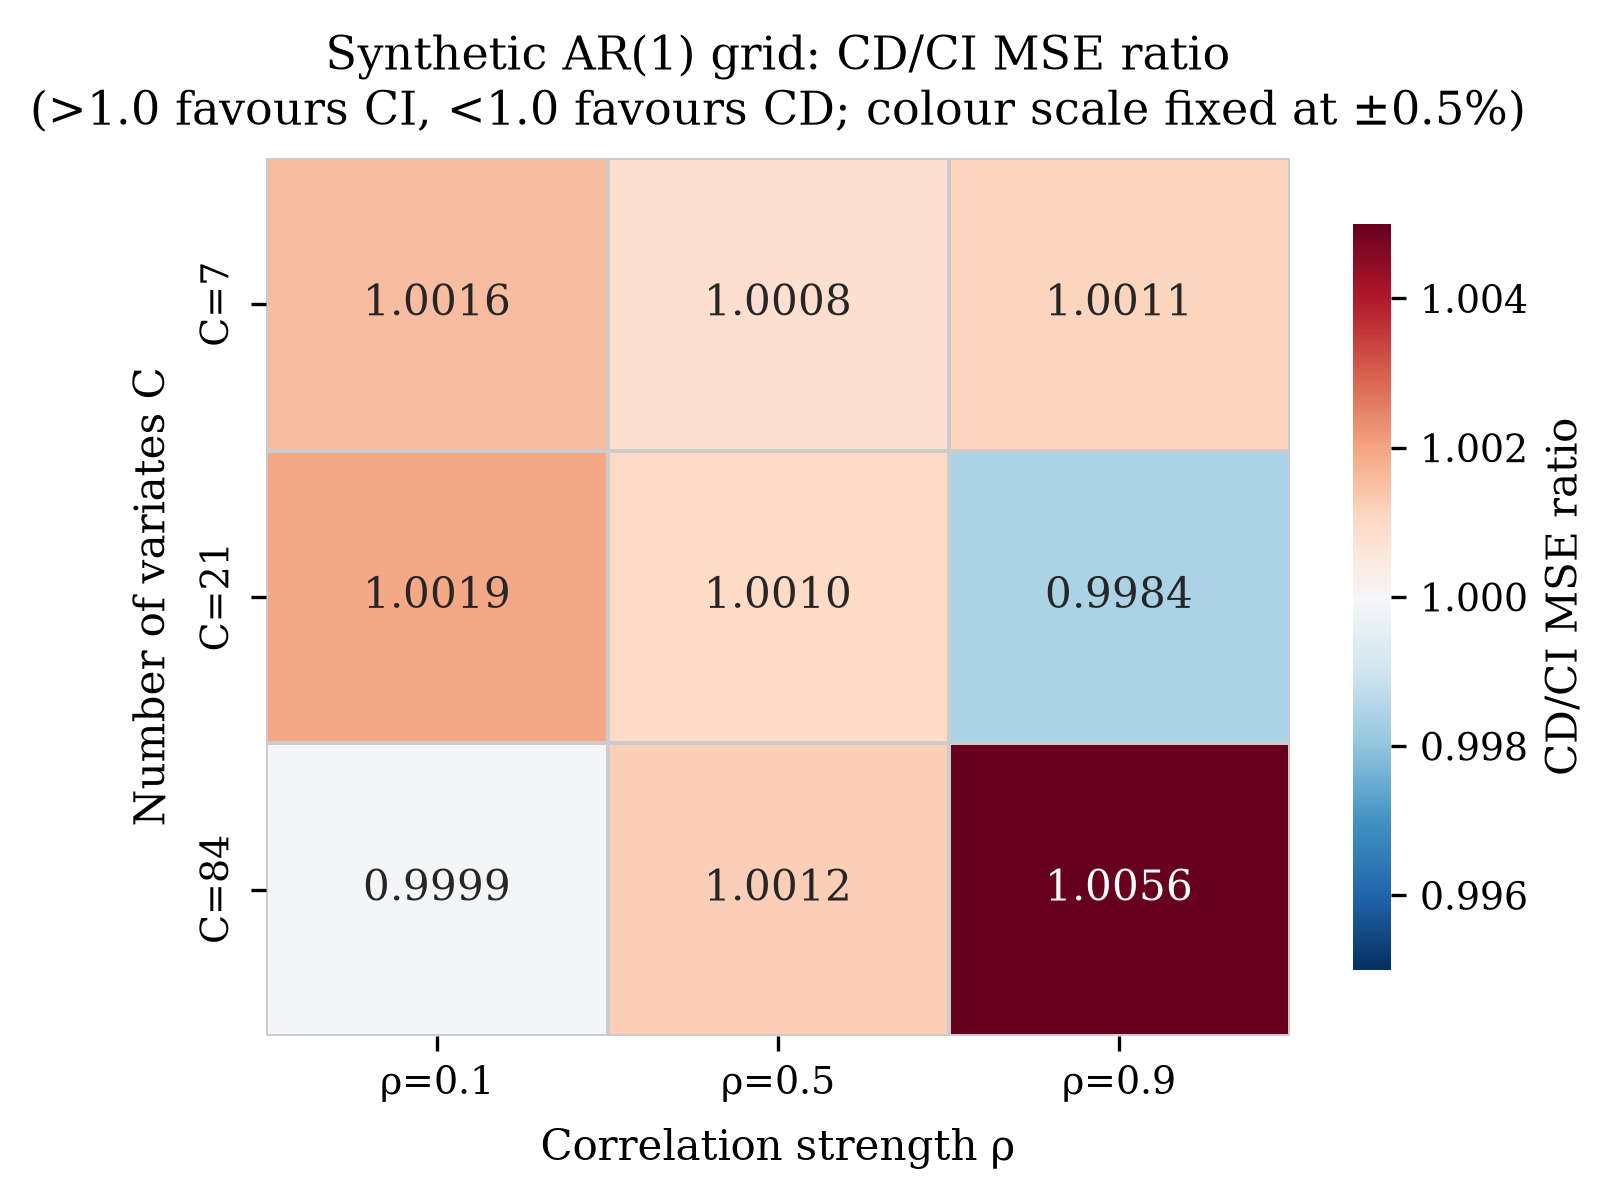
\includegraphics[width=0.75\textwidth]{heatmap.png}
        \caption{Synthetic AR(1) grid: CD/CI test-MSE ratio by variate count $C$ and contemporaneous correlation $\rho$,
            averaged over seeds $\{42, 123, 456, 789, 1011\}$. Values above 1.0 favour CI, below 1.0 favour CD; the
            colour scale is fixed at $\pm 0.5\%$. No cell departs from unity by more than $0.56\%$, and the sign of
            the deviation is not consistent across the grid.}
        \label{fig:synthetic_heatmap}
    \end{figure}

    The $C = 84$, $\rho = 0.9$ cell deserves closer attention. Seeds 42, 123, and 456 all stopped at best epoch 1 or 2
    (7433 / 14866 / 7433 total gradient updates), while CI stopped with only 233--466 updates. At $n = 5$, CD mean is
    0.9813 and CI mean is 0.9759. CD therefore consumed up to $32\times$ more compute per epoch and more epochs before stopping,
    yet landed at essentially the same test MSE. At $\rho \in \{0.1, 0.5\}$ at $C = 84$, CD consistently stops earlier
    than CI while CI takes 9--28 epochs. The two modes follow very different optimisation trajectories yet
    converge to the same test MSE: the extra gradient updates buy CD nothing absent a lagged cross-channel signal for the
    attention to act on.

    \textbf{Statistical analysis.} For each $(C, \rho)$ cell we compute the per-seed difference
    $d_s = e^{\text{CD}}_s - e^{\text{CI}}_s$ over seeds $\{42, 123, 456, 789, 1011\}$ and derive its mean, standard
    deviation, and 95\% confidence interval from a $t$-distribution with four degrees of freedom ($t_{0.025,4} = 2.776$).
    Across all nine cells the mean CD$-$CI difference stays within $\pm 0.0054$ MSE units, at most $0.56\%$ of the
    corresponding CI mean, and seven of nine 95\% CIs include zero. The two that exclude zero are at $C = 7$, $\rho = 0.1$
    and $C = 21$, $\rho = 0.1$; both are positive (CD worse) and below $0.20\%$ of the CI mean in their respective cells,
    well within the detection bound. Pooling the 45 matched pairs as a simple unweighted average over all differences, the
    grand-mean CD$-$CI is $+0.0013$ MSE (95\% CI $[-0.0002, +0.0028]$, $0.13\%$ of the mean CI MSE), and regressing the
    paired difference on $C$ (categorical) and $\rho$ finds no dependence on either factor ($F$-test $p = 0.81$,
    $R^2 = 0.02$). These intervals are a bound rather than a mere failure to reject: pooling the within-cell variances
    gives a 95\% CI half-width of 0.0063 MSE at $n = 5$, roughly $0.63\%$ of the mean CI MSE. Any uniform CD advantage
    larger than $0.63\%$ of the CI mean would have pushed the grand-mean CI entirely above zero; none of the observed
    differences reached that threshold.

    \subsection{Real-Data Experiments}

    \paragraph{ETTh1 ($C = 7$).} Under the matched-budget protocol, CI matches or beats CD at every horizon
    (Table~\ref{tab:etth1}). CD is significantly worse at $H = 96$ (paired 95\% CI $[+0.0013, +0.0618]$) and $H = 720$
    (95\% CI $[+0.0041, +0.0367]$); the $H = 192$ and $H = 336$ differences are not significant. Pooled across all 20
    pairs (four horizons, five seeds), the CD$-$CI difference is $+0.0147$ MSE (95\% CI $[+0.0047, +0.0246]$). The
    $H = 192$ ratio sits below one (CD 0.5194 vs.\ CI 0.5229), the only horizon where CD leads, but the 95\% CI
    $[-0.0227, +0.0159]$ includes zero and CD's lead is not reliable. Steps per epoch are identical across modes at every
    horizon, so neither the update count nor the warmup schedule can explain the CI advantage at the significant horizons.


    \begin{table}[H]
        \centering
        \caption{ETTh1 mean test MSE over seeds $\{42, 123, 456, 789, 1011\}$, matched-budget protocol
            (batch 32, warmup 10, min epochs 15 for both modes). CD/CI above 1.0 favours CI.
            SIG = paired 95\% CI excludes zero.}
        \label{tab:etth1}
        \begin{tabular}{crrrc}
            \toprule
            $H$ & CI     & CD     & CD/CI  &     \\
            \midrule
            96  & 0.4599 & 0.4914 & 1.0686 & SIG \\
            192 & 0.5229 & 0.5194 & 0.9935 &     \\
            336 & 0.5789 & 0.5890 & 1.0174 &     \\
            720 & 0.7062 & 0.7266 & 1.0289 & SIG \\
            \bottomrule
        \end{tabular}
    \end{table}

    \paragraph{ECL ($C = 321$).} Both modes train at this scale under the single-T4 budget (Section~\ref{sec:setup});
    what differs is cost. The accuracy comparison is deliberately narrow, one seed (456) at $H \in \{96, 336\}$, and is
    reported descriptively with no confidence intervals (Table~\ref{tab:ecl}). CD trails CI at both horizons, by $+0.0133$
    MSE ($+7.6\%$ of the CI value) at $H = 96$ and $+0.0113$ ($+5.6\%$) at $H = 336$, and reaches its validation minimum
    far earlier (epochs 13 and 7 against CI's 42 and 25), the same early-minimum shape documented at the synthetic
    $\gamma = 0.6$ cell (Section~\ref{subsec:overtrain}). ECL is included as evidence of this formulation's cost asymmetry
    at scale rather than as a performance benchmark; a single seed supports no significance claim, and we make none.

    \begin{table}[H]
        \centering
        \caption{ECL test MSE, CI versus CD at seed 456, $H \in \{96, 336\}$. Single seed, descriptive only; no
        confidence intervals are reported. Rel is CD$-$CI as a percentage of the CI value.}
        \label{tab:ecl}
        \begin{tabular}{crrrr}
            \toprule
            $H$ & CI     & CD     & CD$-$CI   & Rel      \\
            \midrule
            96  & 0.1753 & 0.1886 & $+0.0133$ & $+7.6\%$ \\
            336 & 0.2037 & 0.2150 & $+0.0113$ & $+5.6\%$ \\
            \bottomrule
        \end{tabular}
    \end{table}

    \begin{figure}[H]
        \centering
        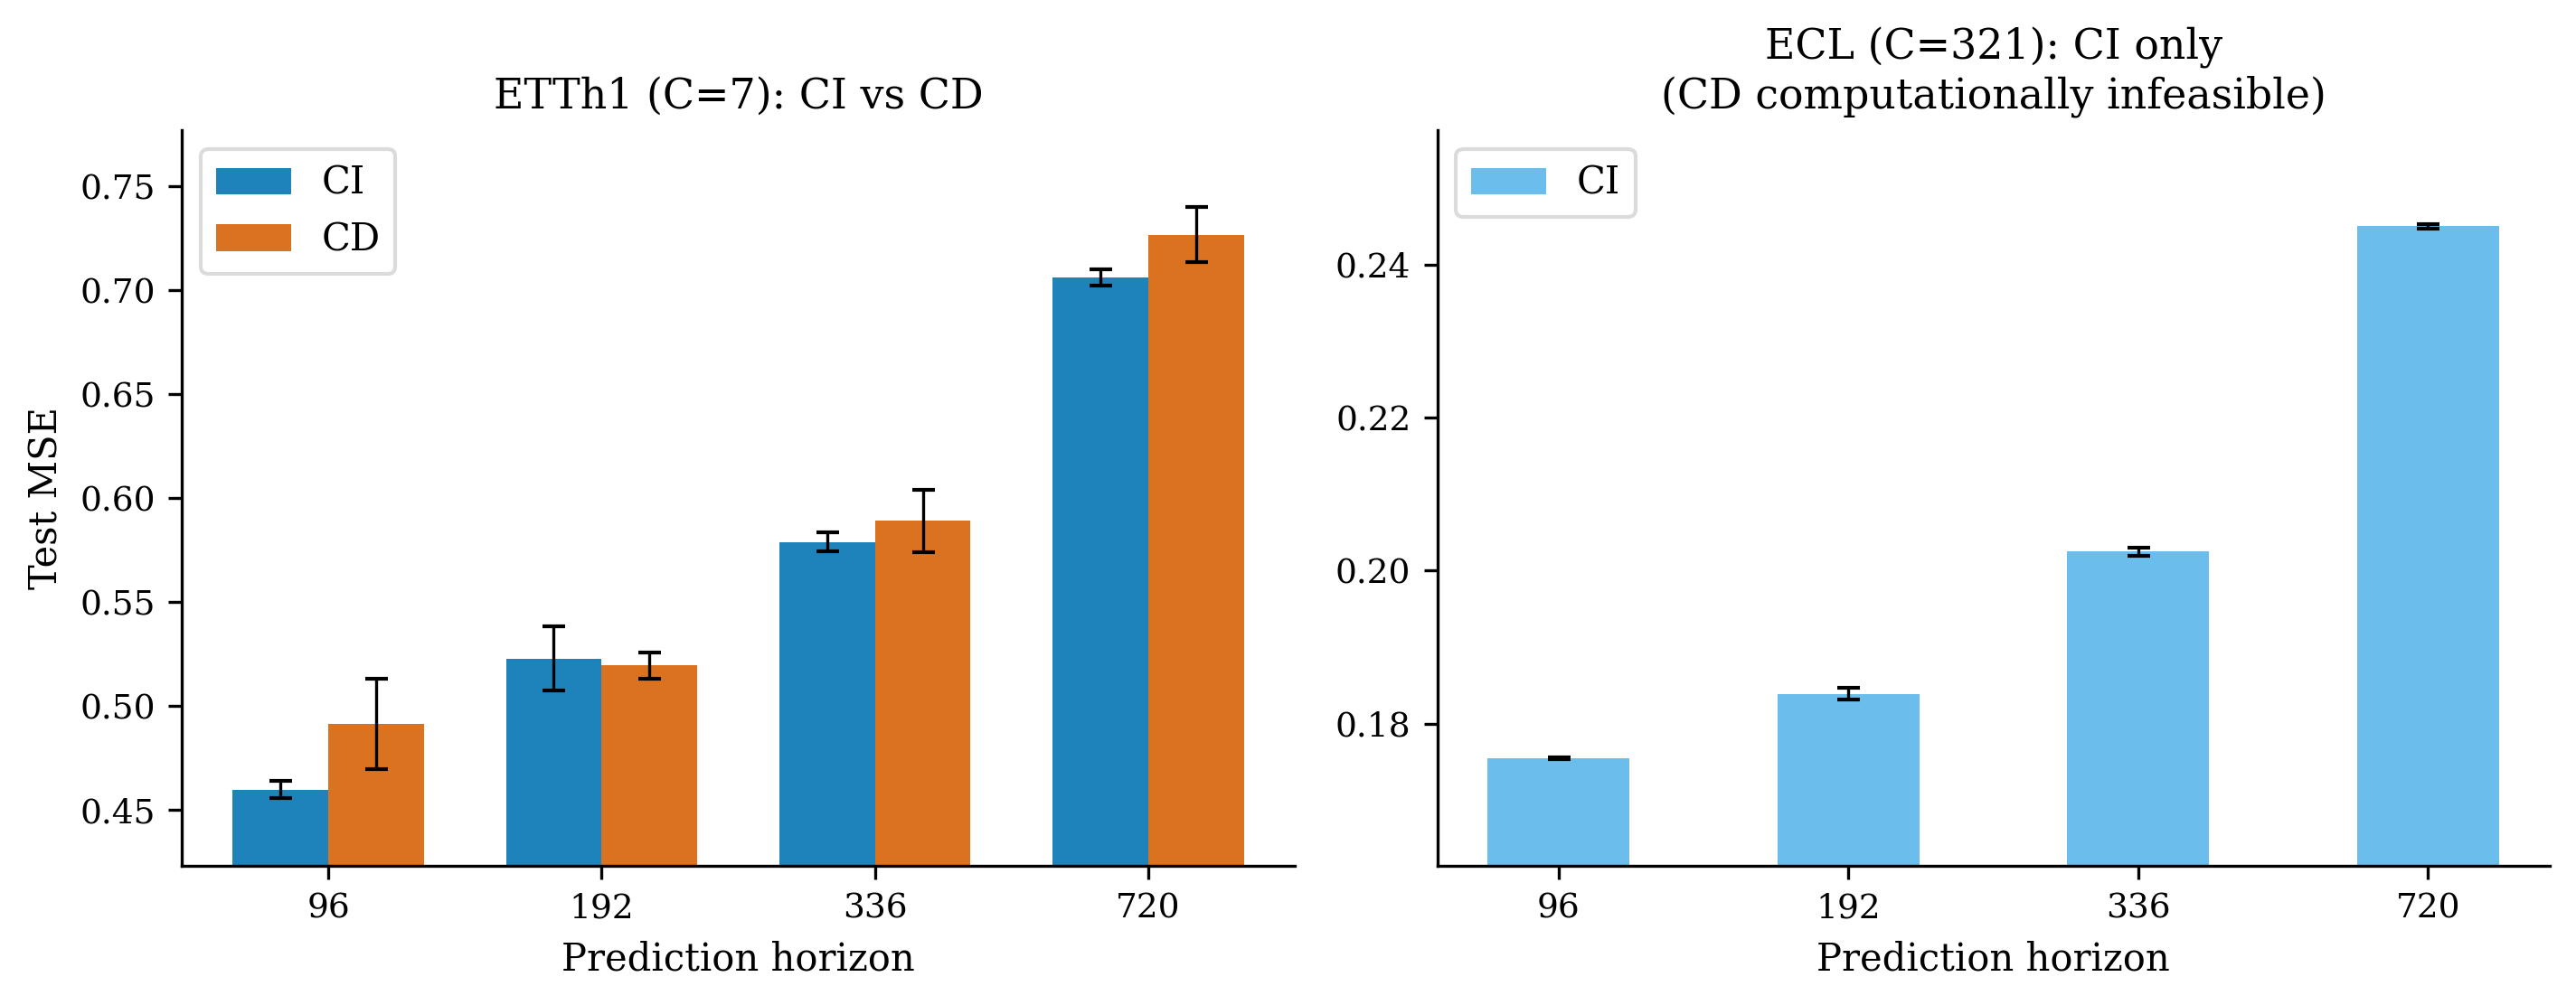
\includegraphics[width=0.85\textwidth]{real_data.png}
        \caption{Real-data test MSE by prediction horizon. Left: ETTh1 ($C = 7$) across $H \in \{96, 192, 336, 720\}$,
        CI versus CD under the matched-budget protocol, mean over seeds $\{42, 123, 456, 789, 1011\}$ with error bars
        showing the cross-seed standard deviation; CI is significantly better at $H \in \{96, 720\}$ and never worse.
        Right: ECL ($C = 321$), CI versus CD at $H \in \{96, 336\}$, single seed (456); no error bars are drawn for
        single-seed groups.}
        \label{fig:real_data}
    \end{figure}

    \paragraph{Correlation and lead-lag structure.} For ETTh1, the lag-0 mean absolute Pearson correlation is 0.311 (median
    0.233) and the mean of each pair's maximum absolute correlation over lags is 0.349; 43\% of channel pairs gain at least
    5 percentage points of absolute correlation from some non-zero lag. For ECL the corresponding numbers are higher: lag-0
    mean 0.503 (median 0.483), mean max-over-lags 0.596, and 49\% of pairs gaining at least 5pp from non-zero lags. In both
    datasets lag~0 is the strongest single lag, but lagged structure adds meaningful signal for a substantial fraction of
    pairs.

    Both datasets sit between the AR(1) grid (instantaneous correlation only) and the leader-follower regime (explicit
    structural lagged coupling). The ETTh1 and ECL results are contextual evidence about CD/CI behaviour in realistic
    settings, not controlled tests of the coupling-structure hypothesis.


    \section{Analysis: Leader-Follower Coupling Experiments}
    \label{sec:analysis}

    The AR(1) null result is easy to explain: when the data has no lagged cross-channel
    signal by construction, a model attending across channels has nothing additional to exploit beyond
    what channel-independent attention already sees. RQ2 asks whether this changes under structured lagged coupling.

    \subsection{Leader-Follower VAR(1) Design}

    We generate data from a $C = 21$ VAR(1) process with the following channel structure: channels 0--9 are \emph{leaders}
    (pure AR(1), no cross-channel dependence); channels 10--19 are \emph{followers}, where follower $i+10$ depends on
    leader $i$ with lag-1 coefficient $\gamma$; channel 20 is an \emph{isolate} (pure AR(1), internal negative control).
    The transition matrix $A(\gamma)$ is lower-triangular with diagonal entries $\phi = 0.8$ and off-diagonal entries
    $A[i+10, i] = \gamma$ for $i \in \{0,\ldots,9\}$. Lower-triangular structure guarantees spectral radius $\phi$ at all
    finite $\gamma$, so the process is stationary by construction.

    At $\gamma = 0$ the process reduces to the original AR(1) grid at $C = 21$, $\rho = 0.5$, providing a cross-experiment
    sanity check. This anchor applies to the $\gamma$-sweep only: the $(P, \gamma)$ boundary sweep uses a different
    generator (Table~\ref{tab:synth_protocols}), so its $\gamma = 0$ cells are not expected to reproduce the AR(1) grid
    and should not be read as a failed check when they do not. We sweep $\gamma \in \{0.0, 0.3, 0.6, 0.9\}$ with five
    seeds and CI, CD, and DLinear modes, all at patch size $P = 16$.

    \subsection{Patch-Resolution Sweep}

    The null result at $P = 16$ has a natural mechanistic explanation: with stride $S = 8$, each patch spans 16 timesteps.
    A lag-1 cross-channel relationship means follower $i+10$ at time $t$ depends on leader $i$ at time $t-1$. Both timesteps
    likely fall within the same patch, but whether the cross-variate attention can resolve a single-step offset within a
    16-timestep window is unclear. Smaller patches would place lag-1 coupling more prominently within the patch structure
    and give CD's attention a more concentrated signal.

    We therefore run a joint sweep over $\gamma \in \{0.0, 0.3, 0.6, 0.9\}$ and $P \in \{2, 4, 8, 16\}$ with $S = P/2$
    (50\% overlap), modes CI and CD, five seeds. At $P = 2$, each patch spans exactly two timesteps and stride $S = 1$, so
    a lag-1 relationship falls across adjacent patches, the finest resolution the architecture supports. CD at
    $P = 4$ was not run in earlier tranches under an assumed VRAM ceiling at this sequence length
    ($C \cdot N = 21 \times 255 = 5355$ tokens); a dedicated boundary tranche, launched to test that assumption directly,
    trains CD successfully at $P = 4$ under the same single-device T4 budget, with full five-seed coverage now complete
    across all four $\gamma$ (Table~\ref{tab:boundary}).

    \subsection{Results}

    Table~\ref{tab:lf_p16} reports mean CI, CD, and DLinear MSE at $P = 16$ across the $\gamma$ sweep ($C = 21$,
    $\text{pred\_len} = 96$, five seeds). The CD/CI ratio stays within $1\%$ of unity throughout and never falls below it,
    but it does climb with $\gamma$ under this early-stopping protocol: regressing the paired CD$-$CI difference on $\gamma$
    gives a slope of $+0.0072$ MSE per unit $\gamma$ (95\% CI $[+0.0027, +0.0117]$, $p = 0.004$, $R^2 = 0.38$). That climb sits
    inside the $1\%$ band at every $\gamma$. Section~\ref{subsec:overtrain} examines the $\gamma = 0.6$ cell directly and
    finds the gap is not produced by checkpoint selection, and that it is small relative to run-to-run variation at five seeds.
    DLinear stays within 0.004 MSE of CI at every $\gamma$, so at this $C$ a channel-independent linear map is about as accurate
    as patch attention, though Table~\ref{tab:synthetic} shows the parity breaks at larger $C$ or $\rho$. These DLinear runs
    reached the epoch budget without early stopping and should be read as budget-limited reference points rather than
    fully converged optima.

    \begin{table}[H]
        \centering
        \caption{Leader-follower VAR(1) at $P = 16$. Mean test MSE and CD/CI ratio over seeds
            $\{42, 123, 456, 789, 1011\}$. CI and CD match the AR(1) grid at $\gamma = 0.0$ to within seed variance.
            The CD/CI ratio stays within $1\%$ of unity across $\gamma$; under this early-stopping protocol it drifts
            upward with $\gamma$, an effect Section~\ref{sec:robustness} finds is not produced by checkpoint
            selection and is small relative to run-to-run variation.}
        \label{tab:lf_p16}
        \begin{tabular}{crrrr}
            \toprule
            $\gamma$ & CI     & CD     & DLinear & CD/CI  \\
            \midrule
            0.0      & 1.0270 & 1.0287 & 1.0301  & 1.0016 \\
            0.3      & 1.0326 & 1.0393 & 1.0330  & 1.0065 \\
            0.6      & 1.0298 & 1.0377 & 1.0301  & 1.0077 \\
            0.9      & 1.0278 & 1.0362 & 1.0284  & 1.0082 \\
            \bottomrule
        \end{tabular}
    \end{table}

    Table~\ref{tab:boundary} shows the CD/CI ratio across the $(P, \gamma)$ grid. At $P \in \{4, 8, 16\}$ the entry is a
    genuine CD/CI ratio. At $P = 2$ CD remains infeasible, so the cell carries the CI-only test MSE where a run exists
    and a dash otherwise ($P = 2$ at $\gamma \in \{0.0, 0.3\}$ was not run under compute constraints). At $P = 4$, CD is
    now feasible and complete across all four $\gamma$, so every cell carries a genuine CD/CI ratio, as at
    $P \in \{8, 16\}$. This joint sweep
    is a separate set of runs from the $\gamma$-sweep in
    Table~\ref{tab:lf_p16}, and it uses a different data-generating protocol: iid innovations, $T = 20{,}000$, and a
    70/10/20 split, against the $\gamma$-sweep's compound-symmetry innovations at $\rho = 0.5$, $T = 14{,}400$, and
    60/20/20 split (Table~\ref{tab:synth_protocols}). Its $P = 16$ ratios sit nearer 1.001 than the 1.007 reported there.
    Because no $P = 16$ cell was run under both generators, the protocol difference and per-seed variation cannot be
    separated with the runs available, and we do not claim to have attributed the gap to either. We therefore do not treat
    the two experiments as independent replications. What they jointly support is the weaker and sufficient claim that the
    CD/CI ratio at $P = 16$ stays within $1\%$ of unity under both protocols.

    \begin{table}[H]
        \centering
        \caption{CD/CI MSE ratio in the $(P, \gamma)$ boundary experiment. At $P \in \{4, 8, 16\}$ both modes run and the
        entry is a CD/CI ratio (above 1.0 favours CI). At $P = 2$ CD exceeds T4 memory, so no ratio is
        defined; those cells carry the CI-only test MSE where a run exists and a dash where none was performed.}
        \label{tab:boundary}
        \begin{tabular}{crrrr}
            \toprule
            $P$ & $\gamma = 0.0$ & $\gamma = 0.3$ & $\gamma = 0.6$ & $\gamma = 0.9$ \\
            \midrule
            16  & 1.0012         & 1.0004         & 1.0005         & 1.0010         \\
            8   & 1.0014         & 1.0009         & 1.0009         & 1.0004         \\
            4   & 0.9997         & 1.0004         & 1.0002         & 1.0004         \\
            2   & ---            & ---            & CI: 0.9806     & CI: 0.9801     \\
            \bottomrule
        \end{tabular}
    \end{table}

    \begin{figure}[H]
        \centering
        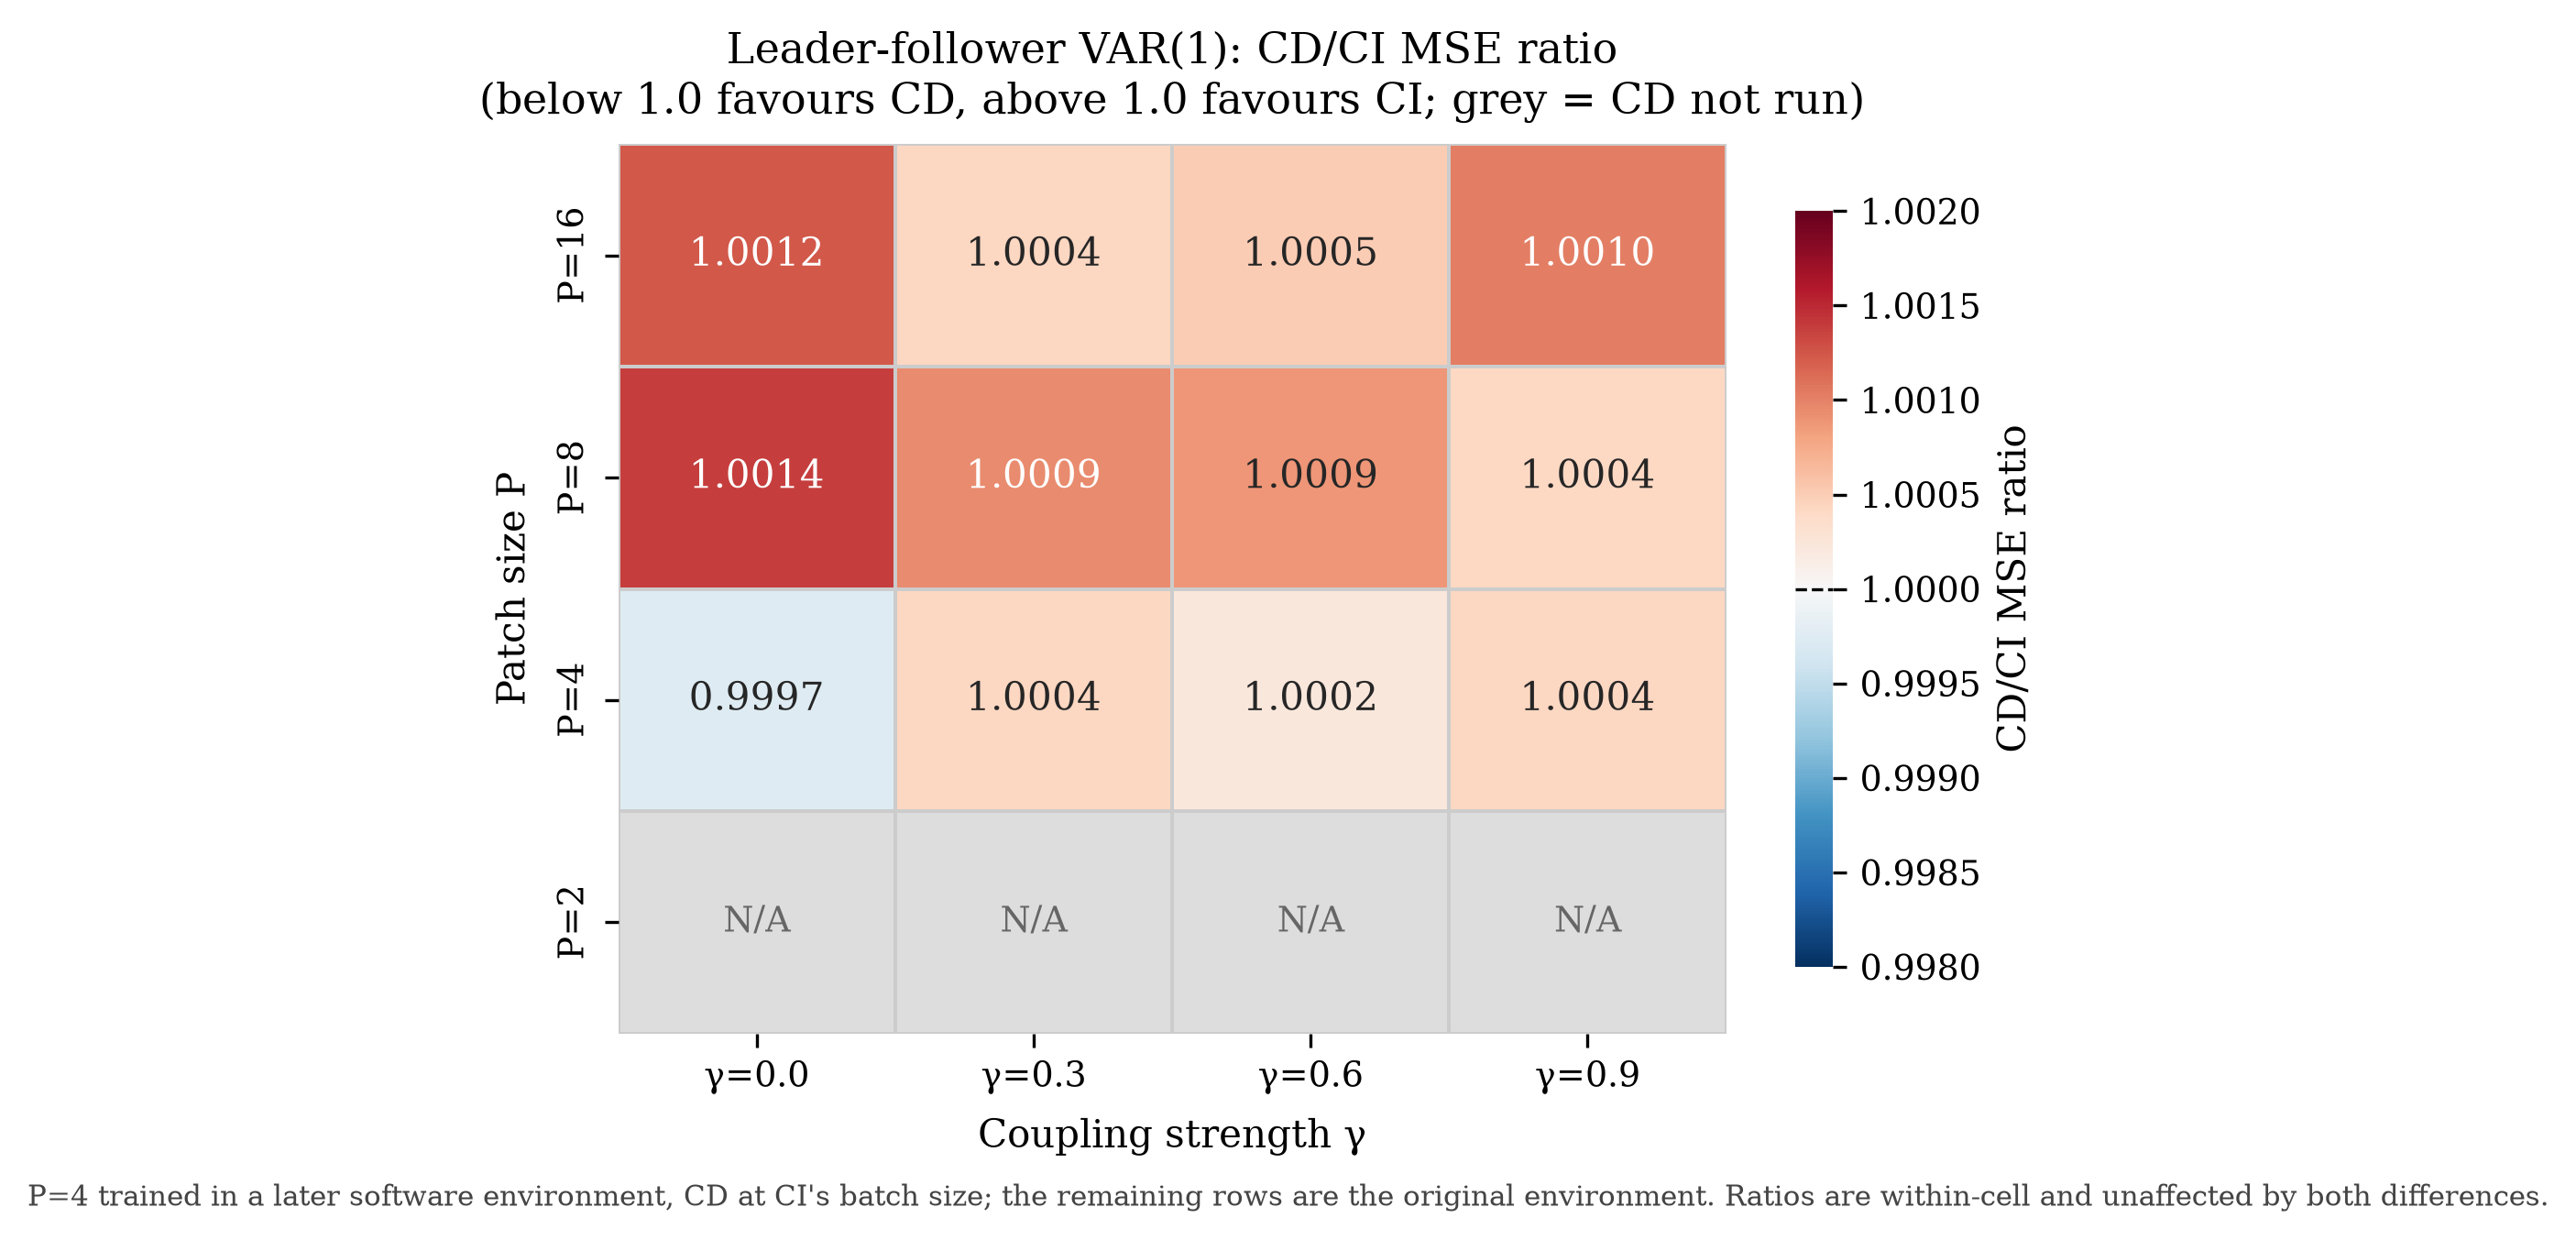
\includegraphics[width=0.75\textwidth]{boundary_heatmap.png}
        \caption{Leader-follower VAR(1): CD/CI test-MSE ratio across the $(P, \gamma)$ grid, mean over seeds
            $\{42, 123, 456, 789, 1011\}$. Values above 1.0 favour CI. Coloured cells are the configurations where both modes were
            run ($P \in \{4, 8, 16\}$); the grey cells at $P = 2$ mark where CD exceeds T4 memory and was not run. Eleven of
            the twelve coloured cells favour CI and one ($P = 4$, $\gamma = 0.0$) falls marginally below unity at $0.9997$;
            the ratio stays within $0.15\%$ of unity throughout.}
        \label{fig:boundary_heatmap}
    \end{figure}

    \subsection{Block-wise Attention Ablation}
    \label{subsec:block_attn}

    The results above use a CD encoder attending over all $C\cdot N$ tokens. A residual question is whether the null result
    depends on that unrestricted scope, or would hold even under an encoder that can only attend within the coupled leader-follower
    pairs. We implement a block-wise variant (CD\_Block) that restricts attention to each leader-follower pair, treating
    the isolate channel as a singleton; this is the minimum scope under which a block-wise encoder can express the lag-1
    coupling under study, and the implementation is parameter-matched to vanilla CD so any difference is attributable to
    attention scope alone. We train it alongside same-environment CI and CD arms across the full $\gamma$ sweep, five
    seeds each.

    Table~\ref{tab:block_attn} reports the three-arm comparison. Across $\gamma > 0$ the block-wise variant sits
    between the two reference arms: CD\_Block/CI ranges 1.0045--1.0056 against CD/CI's 1.0065--1.0082. The paired
    CD\_Block$-$CI difference is not reliably distinguishable from zero at any $\gamma$ (95\% CIs span
    $[-0.0018,+0.0111]$ at $\gamma=0.3$ through $[-0.0005,+0.0119]$ at $\gamma=0.9$), while paired CD\_Block$-$CD
    differences are negative at every $\gamma$ (narrowing vanilla CD's deficit) though individually not significant
    either. Restricting attention to within-pair blocks therefore narrows but does not close vanilla CD's cost-free
    deficit against CI: at five seeds per cell the block variant is neither distinguishable from CI nor confidently
    different from vanilla CD, so we report it as intermediate rather than extending the practical-equivalence
    conclusion to it with the same certainty as the arms in Table~\ref{tab:equiv}.


    \begin{table}[H]
        \centering
        \caption{Leader-follower VAR(1) at $P = 16$: block-wise cross-variate attention (CD\_Block) alongside CI and
            CD. CD\_Block restricts attention to leader-follower pairs (isolate as singleton), parameter-matched to
            vanilla CD. Mean test MSE over seeds $\{42, 123, 456, 789, 1011\}$.}
        \label{tab:block_attn}
        \begin{tabular}{crrrrrr}
            \toprule
            $\gamma$ & CI     & CD     & CD\_Block & CD/CI  & Blk/CI & Blk/CD \\
            \midrule
            0.0      & 1.0270 & 1.0287 & 1.0273    & 1.0016 & 1.0003 & 0.9986 \\
            0.3      & 1.0326 & 1.0393 & 1.0372    & 1.0065 & 1.0045 & 0.9980 \\
            0.6      & 1.0298 & 1.0377 & 1.0353    & 1.0077 & 1.0054 & 0.9977 \\
            0.9      & 1.0278 & 1.0362 & 1.0335    & 1.0082 & 1.0056 & 0.9974 \\
            \bottomrule
        \end{tabular}
    \end{table}

    The same three-arm design extends to the AR(1) grid at $C = 84$, $\rho = 0.5$, where the flattened sequence reaches
    $C \cdot N = 5{,}292$ tokens and the grouping (28 contiguous blocks of 3) is necessarily neutral, since
    compound-symmetry covariance has no block structure to align with. These runs use a later training environment in
    which CD and CD\_Block fit at batch 8 rather than the main grid's batch 1, and a fresh five-seed data generation at
    14{,}400 timesteps, so the cell is self-contained and is never paired row-by-row against Table~\ref{tab:synthetic}.
    All three arms land together: mean test MSE 1.0076 (CI), 1.0045 (CD), 1.0050 (CD\_Block); paired CD$-$CI is
    $-0.0031$ ($-0.31\%$ of the CI mean, 95\% CI $[-0.0105, +0.0042]$), CD\_Block$-$CI is $-0.0027$
    ($[-0.0093, +0.0039]$), and CD\_Block$-$CD is $+0.0005$ ($[-0.0022, +0.0032]$), every interval spanning zero. The
    point estimates all sit inside the $1\%$ band; the CD$-$CI interval's lower edge reaches $-1.04\%$ of the CI mean,
    marginally past the band on the CD-favourable side, which we state rather than round away. CD-family validation
    minima again fall early, at epochs 6--10 against CI's 9--17.


    \subsection{Mechanistic Interpretation}
    \label{subsec:mechanistic}

    The two leader-follower experiments differ in how sensitive the gap looks to $\gamma$. The boundary sweep gives a flat
    trend (slope $-0.0006$ MSE per unit $\gamma$, 95\% CI $[-0.0021, +0.0009]$, $p = 0.44$, $n = 5$), whereas the dedicated
    $P = 16$ sweep shows a larger apparent trend under the original early-stopping protocol. The slope is fitted on
    $P \in \{8, 16\}$ only: the $P = 4$ cells were trained in a later software environment in which CD ran at CI's batch
    size rather than at batch 8, so pooling them into one slope would confound the coupling effect with both differences.
    Their within-cell CD/CI ratios, which neither difference affects, appear in Table~\ref{tab:boundary}. The
    environment difference itself is small and measured: re-running the CI arm at $P = 4$ in the later environment moves
    the per-$\gamma$ CI mean by $+0.0002$ ($\gamma = 0.6$) and $+0.0006$ ($\gamma = 0.9$), well inside the
    old-environment 95\% half-widths of 0.0268 and 0.0301.
    A seed-clustered version of the same regression, treating each seed as a cluster, gives an equally flat slope
    (95\% CI $[-0.0029, +0.0018]$, $p = 0.62$), so the result does not depend on treating seeds as independent.
    They agree that CD never holds a practically relevant lead; they differ on whether the gap drifts with $\gamma$.
    Section~\ref{sec:robustness} bears on this difference without settling it. The dedicated sweep's trend is not produced
    by checkpoint selection (Section~\ref{subsec:overtrain}), and at $\gamma = 0.6$ the deficit is comparable in size to
    the run-to-run spread across reruns of that cell. The part of the gap that does track $\gamma$ is a property of the
    shared prediction head rather than the encoder (Section~\ref{subsec:cdhead}). These are two separate findings, each
    supported by its own experiment, and we do not use either to stand in for the other.

    A representational reading of why CD gains nothing from the coupling is also available. At $P = 16$ and $S = 8$, a
    lag-1 cross-channel relationship maps to the same patch position in both the leader and the follower sequence rather
    than to a phase offset between them, so the cross-variate attention has no distinct inter-patch signal to route:
    position $k$ of variate $j+10$ sits beside position $k$ of variate $j$ in the
    $C \cdot N = 21 \times 63 = 1323$-token sequence, but the lag-1 information is already aggregated within the shared
    patch position. CD and CI test MSEs stay within seed variance in every cell where both modes run
    ($P \in \{4, 8, 16\}$). The finest resolution, $P = 2$ with stride 1, where lag-1 coupling would fall across adjacent
    patches and a phase offset would be visible, is CI-only because CD exceeds T4 memory there. This account therefore
    cannot be tested directly and remains a conjecture rather than a result.


    \section{Fair-Protocol Robustness Controls}
    \label{sec:robustness}

    The leader-follower $P = 16$ sweep raises a question the main protocol cannot answer on its own: the apparent
    CD$-$CI gap grows with $\gamma$ (Section~\ref{sec:analysis}), which could mean CD is genuinely worse under stronger
    coupling, or could mean the training protocol places CD at a disadvantage. This section tests both readings with four
    analyses, covering checkpoint selection, update budget, head design, and covariance structure, and then summarises the
    resulting effect sizes against a pre-specified threshold. The first returns a negative result and we report it as
    such: checkpoint selection does not explain the gap. We fix the practical-equivalence threshold at $1\%$ of the CI
    mean test MSE, pre-specified before these analyses were run; differences smaller than this in either direction are
    treated as practically irrelevant regardless of statistical significance. This is an operational cutoff on observed
    effect sizes, not a formal statistical-equivalence claim over the reported confidence intervals.

    \subsection{Overtraining and Selection}
    \label{subsec:overtrain}

    To test whether checkpoint selection explains the gap, we instrument one training run per (mode, seed) at the
    leader-follower $\gamma = 0.6$, $C = 21$ cell, logging validation MSE five times per epoch and training past the
    early-stopping horizon for all five seeds $\{42, 123, 456, 789, 1011\}$. Because mid-epoch validation runs in
    evaluation mode, it draws no random numbers and does not perturb the weight trajectory, so one trajectory supports
    every post-hoc selection rule we compare on that trajectory. Whether it reproduces the original run is a separate
    question, addressed next.

    These are fresh instrumented reruns under the identical protocol (same seeds, same steps per epoch: 1005 for CD, 63
    for CI), not a replay of the original trajectories. They land within one epoch of the original run's best epoch in 6 of 10 runs and within two epochs in the rest. CD's rerun test MSE is lower than its original on all five seeds ($+0.0079$
    MSE, 95\% CI $[+0.0042, +0.0117]$), while CI's difference spans zero ($-0.0019$, 95\% CI $[-0.0084, +0.0046]$). We
    cannot attribute that CD-specific shift with the runs available, and we do not treat the diagnostic as reproducing
    the original numbers.

    What the curves show is overtraining in CD. Across seeds, CD reaches its validation minimum at epoch 4 to 7 and then
    climbs from 0.9865 to 1.1999 MSE by the end of training, while CI reaches its minimum later, at epoch 16 to 20, and
    stays near it (0.9863 to 1.0033). Figure~\ref{fig:diag_overlay} shows the asymmetry. The early-minimum shape recurs
    beyond this cell: in the $C = 84$, $\rho = 0.5$ three-arm run (Section~\ref{subsec:block_attn}) CD-family best epochs
    fall at 6--10 against CI's 9--17, and the single-seed ECL comparison shows the same pattern at $C = 321$
    (Section~\ref{sec:results}).

    What the curves do \emph{not} show is that overtraining produces the gap. The original protocol already restores the
    validation-best checkpoint: in every committed row the recorded total step count equals best epoch times steps per
    epoch, so the reported test MSE is the minimum-validation checkpoint, not the checkpoint at which patience expired.
    Selecting each model at its validation minimum is therefore not a different rule, and on the diagnostic curves the
    two rules select the same checkpoint on every seed, to the last digit. The difference between the original
    $+0.0079$ MSE (95\% CI $[+0.0046, +0.0113]$) and the diagnostic $-0.0031$ MSE (95\% CI $[-0.0109, +0.0046]$)
    decomposes accordingly: epoch-granularity selection contributes exactly zero, the mid-epoch evaluation cadence
    contributes $-0.0012$ paired (CD $+0.0005$, 95\% CI $[-0.0049, +0.0059]$; CI $-0.0007$, 95\% CI
    $[-0.0062, +0.0047]$), and the original runs sit a further $+0.0098$ (95\% CI $[+0.0001, +0.0195]$) above the
    reruns, which separates two run sets rather than two selection rules.

    We therefore withdraw the selection explanation for this cell. The deficit under the original protocol is $+0.77\%$
    of the CI mean, inside the pre-specified band, and the run-to-run spread at five seeds is comparable to the effect
    itself, so we do not read the $\gamma = 0.6$ deficit as a stable architectural quantity. Every selection rule and protocol
    variant we tried at this cell lands inside the pre-specified band, in one direction or the other, with a noise floor
    comparable to the effects themselves, and Section~\ref{sec:theoretical_bound} shows no cross-channel signal is
    available at this horizon to any predictor.

    \begin{figure}[H]
        \centering
        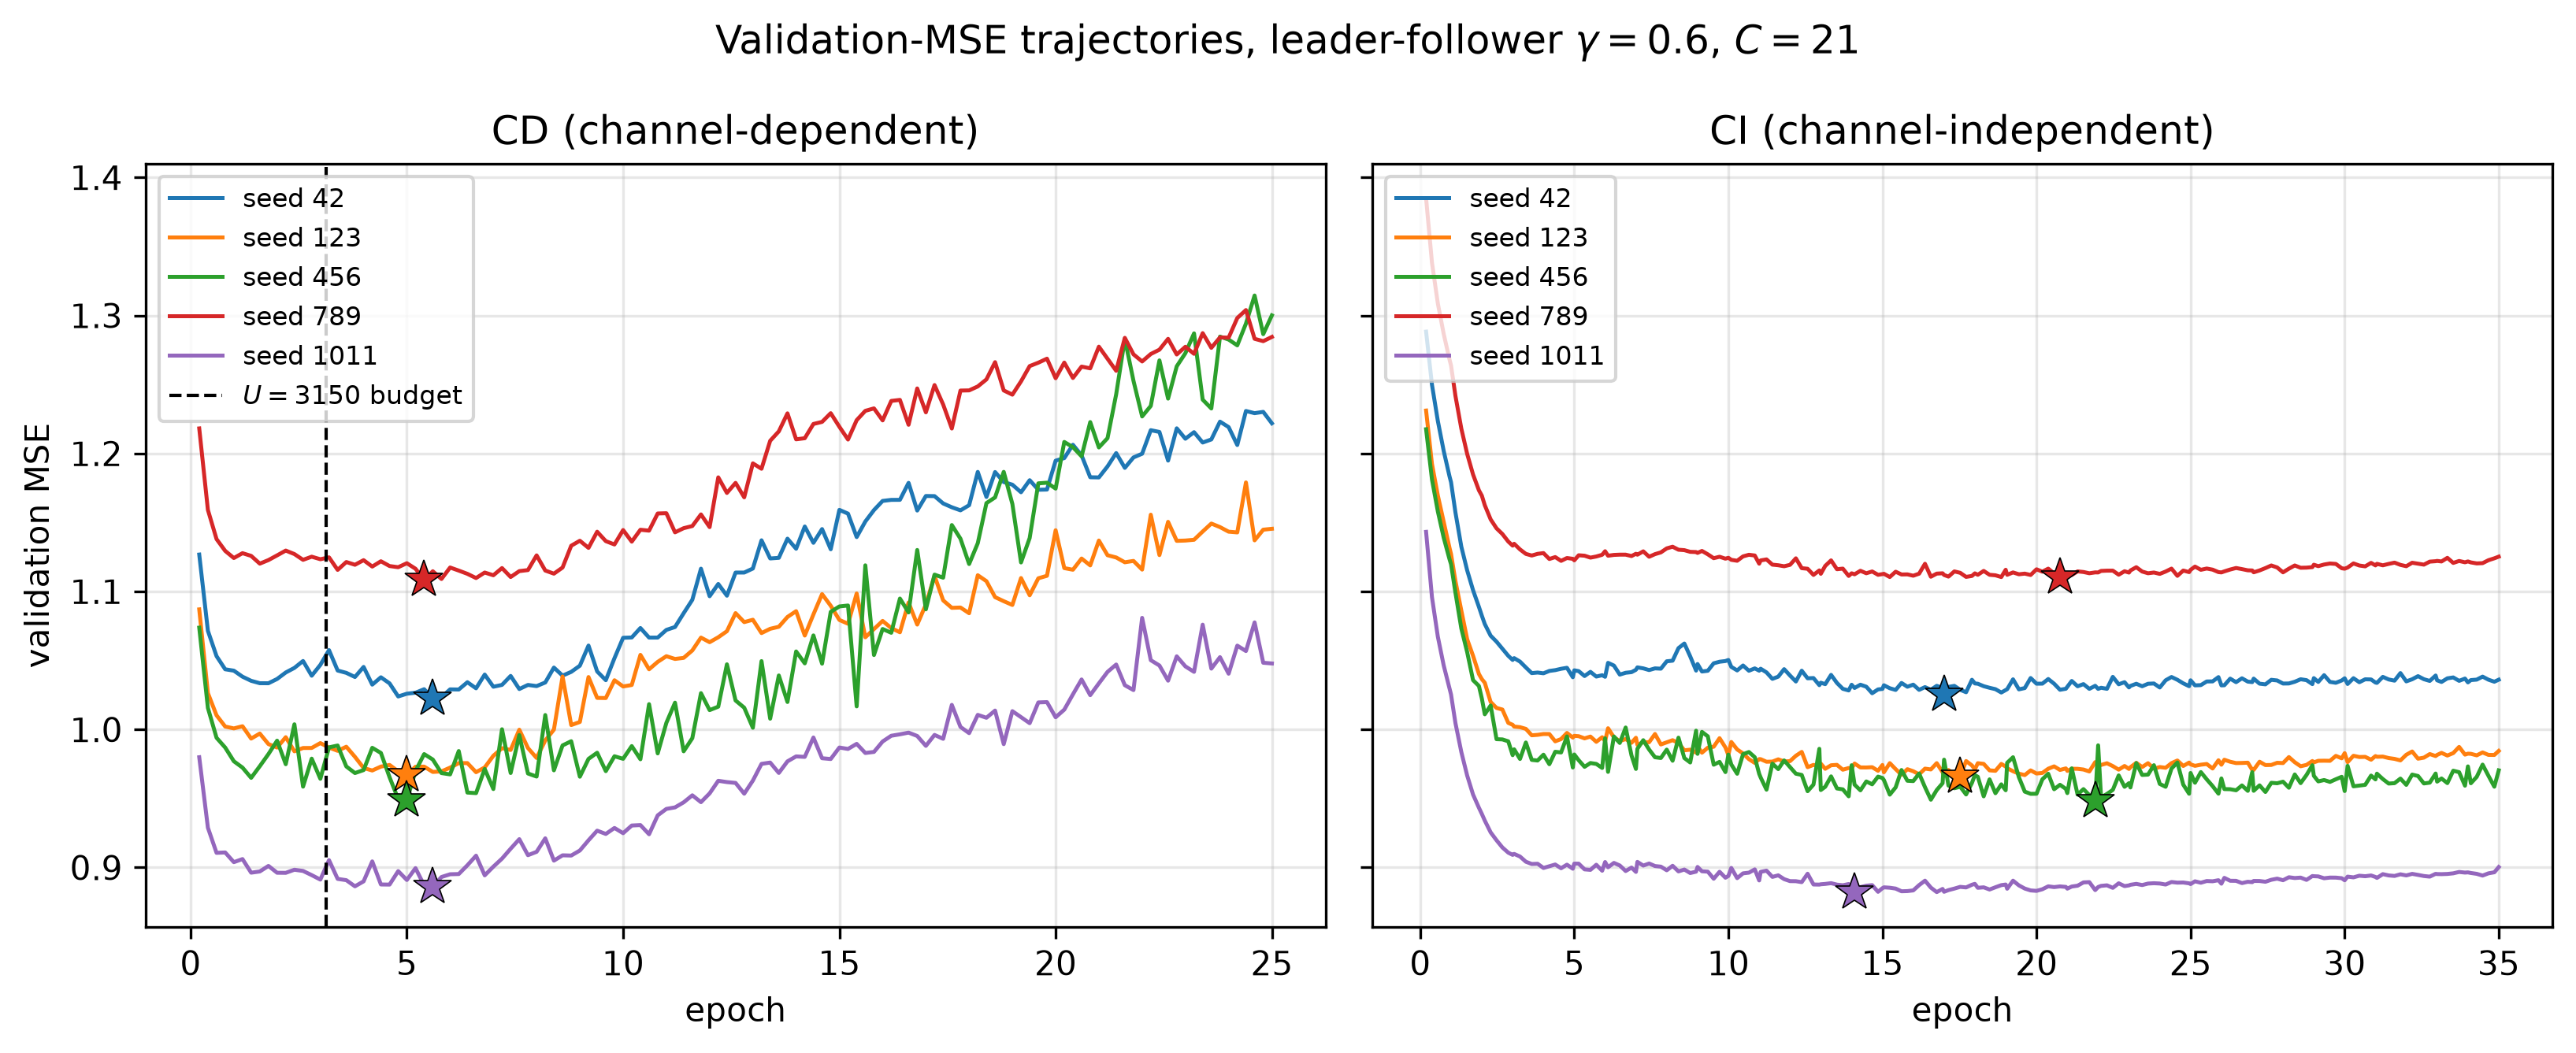
\includegraphics[width=\linewidth]{diag_overlay_clean.png}
        \caption{Validation-MSE trajectories at the leader-follower $\gamma = 0.6$, $C = 21$ cell, one instrumented
            rerun per seed, drawn to each mode's diagnostic horizon. Stars mark each seed's validation minimum. CD
            (left) reaches a sharp minimum near epoch 4 to 7 and then degrades, while CI (right) settles into a flat
            basin. The dashed line on the CD panel marks the matched update budget $U = 3150$, which falls before CD's
            minimum, so a budget-capped rule truncates CD before its best checkpoint.}
        \label{fig:diag_overlay}
    \end{figure}

    \subsection{Matched Update Budget}
    \label{subsec:equalcompute}

    At $C = 21$ the original protocol gives CD many more gradient updates per epoch than CI (Table~\ref{tab:batch_sizes}),
    which invites the objection that CD is simply trained for longer and pushed past its optimum. Capping both modes at an
    identical update budget and taking the best checkpoint within it answers that objection. The deficit does not survive
    the cap: the CD$-$CI difference is $-0.0036$ MSE (95\% CI $[-0.0059, -0.0012]$) at leader-follower $\gamma = 0.0$ and
    $-0.0053$ MSE (95\% CI $[-0.0092, -0.0014]$) at $\gamma = 0.6$, both favouring CD, and $-0.0028$ MSE (95\% CI
    $[-0.0138, +0.0082]$) at the AR(1) $C = 84$, $\rho = 0.9$ cell, a tie. The per-epoch step-count asymmetry is not what
    produces the apparent deficit. We treat this protocol as a sensitivity check rather than a canonical schedule, because
    the budget $U = 3150$ is itself too tight for CD at leader-follower $\gamma = 0.6$: it truncates training before CD's
    validation minimum, and the sign turns positive ($+0.0059$ MSE, 95\% CI $[+0.0003, +0.0114]$). Given the overtraining
    shape documented in Section~\ref{subsec:overtrain}, that is a consequence of where the cap falls rather than a
    separate disadvantage.

    \subsection{Head Fairness}
    \label{subsec:cdhead}

    The CD architecture in the main experiments shares CI's per-variate prediction head, so a residual objection is that the
    head, not the encoder, limits CD. We rerun the leader-follower sweep with a cross-variate head (CD\_Head) that pools
    across variates before projecting, leaving the encoder unchanged. The cross-variate head ties CI at every coupling
    strength: CD\_Head$-$CI is $+0.0016$ ($\gamma = 0.0$), $+0.0030$ ($\gamma = 0.6$), and $+0.0023$ MSE ($\gamma = 0.9$),
    all within $0.3\%$ of the CI mean and all with 95\% CIs spanning zero. Pooled across $\gamma$, the CD\_Head$-$CI grand
    mean is $+0.0023$ MSE ($+0.23\%$ of the CI mean) with a 95\% CI whose lower bound sits just above zero, so the
    cross-variate head is detectably though negligibly worse than CI in pooled terms, well inside the $1\%$ band. The plain
    shared-head CD over the same runs is
    $+0.0017$, $+0.0079$, and $+0.0085$ MSE, carrying the $\gamma$-dependent widening that the main sweep showed. Swapping
    only the head removes that widening while leaving the encoder fixed, which locates the coupling-dependent widening in the
    shared head rather than in the cross-variate encoder. This is a head effect specifically; it is separate evidence from
    the overtraining phenomenon of Section~\ref{subsec:overtrain}, and we do not use one to explain the other.

    \subsection{Covariance Family}
    \label{subsec:blockcov}

    The AR(1) grid uses compound-symmetry covariance, where every channel pair shares the same correlation. To check that
    the null is not specific to that structure, we test a block-covariance family in which within-block correlation
    $\rho_{\text{in}} \in \{0.5, 0.9\}$ is concentrated in groups of seven variates and cross-block correlation is zero,
    giving CD a block structure to exploit that compound symmetry does not offer. CD gains no practically relevant advantage
    there either: at $C = 21$ the CD$-$CI difference is $+0.0028$ MSE ($+0.27\%$, 95\% CI $[+0.0015, +0.0040]$) at
    $\rho_{\text{in}} = 0.5$ and $-0.0062$ MSE ($-0.60\%$, 95\% CI $[-0.0137, +0.0013]$) at $\rho_{\text{in}} = 0.9$; at
    $C = 84$, $\rho_{\text{in}} = 0.5$ it is $+0.0005$ MSE ($+0.05\%$, 95\% CI $[-0.0005, +0.0016]$), and at $C = 84$,
    $\rho_{\text{in}} = 0.9$ it is $+0.0000$ MSE ($+0.00\%$, 95\% CI $[-0.0010, +0.0010]$), a tie. Regressing the paired
    difference on variate count and $\rho_{\text{in}}$ across the four cells gives a significant $\rho_{\text{in}}$ slope
    ($-0.0118$ MSE per unit $\rho_{\text{in}}$, $p = 0.013$, $R^2 = 0.35$), so CD's standing relative to CI improves
    slightly as within-block correlation rises, while variate count carries no effect ($p = 0.26$). Every cell sits within
    the $1\%$ threshold, and the $C = 84$ cells again ran CD at batch size 1.

    \subsection{Practical-Equivalence Summary}
    \label{subsec:equiv_summary}

    Table~\ref{tab:equiv} collects the controlled synthetic effect sizes with the selection rule used for each, so that
    cells evaluated under different protocols are never pooled. Across all tested AR(1), leader-follower, and
    block-covariance cells, the absolute CD$-$CI difference stays within the pre-specified $1\%$ relative-MSE threshold in
    both directions. For the AR(1) grid this holds cell by cell as well as in aggregate: no single cell exceeds $0.56\%$ of
    its CI mean (Section~\ref{sec:results}), so the grand-mean row of Table~\ref{tab:equiv} does not average over any
    cell that breaches the threshold. Some differences are statistically detectable in one direction or the other, but none
    reaches the practical threshold. The conclusion is narrow and symmetric: on these controlled synthetic processes,
    neither mode holds a practically relevant accuracy advantage under fair selection. A related architecture-scope control,
    restricting CD's attention to the coupled leader-follower pairs (Section~\ref{subsec:block_attn}), narrows vanilla
    CD's deficit against CI but is not folded into Table~\ref{tab:equiv}: at five seeds it is not confidently distinguishable
    from either reference arm, so we report it as intermediate rather than as a third practically-equivalent cell.

    \begin{table}[H]
        \centering
        \caption{Controlled synthetic effect sizes, CD$-$CI in test MSE, each with the selection rule under which it was
        computed. Cells under different rules are never pooled. ``Rel'' is the difference as a percentage of the
        CI mean; the final column reports whether the absolute difference stays within the pre-specified $1\%$
            threshold. The $\gamma = 0.6$ early-stop row is from the original runs; the val-minimum row is from the
            instrumented reruns (Section~\ref{subsec:overtrain}), so the two differ in run set as well as rule.}
        \label{tab:equiv}
        \small
        \setlength{\tabcolsep}{3pt}
        \begin{tabular}{lllrr c}
            \toprule
            Family          & Cell                               & Selection rule & CD$-$CI   & Rel       & $\le 1\%$ \\
            \midrule
            AR(1) grid      & grand mean (9 cells)               & early-stop     & $+0.0013$ & $+0.13\%$ & yes       \\
            \midrule
            Leader-follower & $\gamma = 0.6$                     & early-stop     & $+0.0079$ & $+0.77\%$ & yes       \\
            Leader-follower & $\gamma = 0.6$                     & val-minimum    & $-0.0031$ & $-0.30\%$ & yes       \\
            Leader-follower & $\gamma = 0.6$                     & matched-$U$    & $-0.0053$ & $-0.52\%$ & yes       \\
            Leader-follower & $\gamma = 0.9$                     & early-stop     & $+0.0085$ & $+0.82\%$ & yes       \\
            Leader-follower & $\gamma = 0.6$, cross-var.\ head   & early-stop     & $+0.0030$ & $+0.29\%$ & yes       \\
            Leader-follower & $\gamma = 0.9$, cross-var.\ head   & early-stop     & $+0.0023$ & $+0.23\%$ & yes       \\
            \midrule
            AR(1)           & $C{=}84$, $\rho{=}0.9$             & matched-$U$    & $-0.0028$ & $-0.27\%$ & yes       \\
            Block-cov.      & $C{=}21$, $\rho_{\text{in}}{=}0.5$ & early-stop     & $+0.0028$ & $+0.27\%$ & yes       \\
            Block-cov.      & $C{=}21$, $\rho_{\text{in}}{=}0.9$ & early-stop     & $-0.0062$ & $-0.60\%$ & yes       \\
            Block-cov.      & $C{=}84$, $\rho_{\text{in}}{=}0.5$ & early-stop     & $+0.0005$ & $+0.05\%$ & yes       \\
            Block-cov.      & $C{=}84$, $\rho_{\text{in}}{=}0.9$ & early-stop     & $+0.0000$ & $+0.00\%$ & yes       \\
            \bottomrule
        \end{tabular}
    \end{table}


    \section{Theoretical Ceiling on Achievable Accuracy}
    \label{sec:theoretical_bound}

    The empirical near-parity result above raises a natural question: how much accuracy was actually available for CD to
    win. We answer this in closed form from the generative model itself, without additional training
    runs\footnote{Reproducible from \texttt{derive\_theoretical\_bounds.py}, committed alongside the paper's other
    analysis scripts; every value in Table~\ref{tab:theoretical_bounds} regenerates directly from this script against the
    same generator constants used elsewhere in the paper.}. For every
    diagonal-transition family (the AR(1) grid, block-covariance, and boundary-sweep experiments), the argument is exact:
    since innovations are drawn i.i.d.\ across time and the transition matrix carries no cross-channel term, the
    channel-independent predictor attains the same forecast-error variance as a full-information predictor, for any
    innovation covariance. In the paper's z-scored units this reduces to $1 - \phi^{2h}$, independent of $\rho$, $C$, and
    group structure; at $\phi = 0.8$ and $\text{pred\_len} = 96$ this equals 1.0 to float64 precision, indistinguishable
    from no signal.

    The leader-follower design has a non-diagonal transition, so this argument does not apply directly to follower
    channels. Leader and isolate channels receive no incoming coupling and remain diagonal, so their ceiling is exact and
    matches the other families. For followers, both ceilings are available in closed form. The full-information
    (CD-restricted) bound follows directly from the joint state-space model. The own-history (CI-restricted) ceiling
    requires more care, because a follower's past partially reveals its leader's past, so the optimal own-history
    predictor is not the marginal AR(1) predictor: treating the joint process as a state-space model observed through the
    follower channel alone, the steady-state Kalman predictor is optimal over all own-history predictors, and its
    $h$-step error variance is the CI ceiling. The derivation script asserts two exact checks and raises on failure: at
    $\gamma = 0$ the ceiling must reproduce $1 - \phi^{2h}$ at every horizon, and $\text{CD} \le \text{CI} \le 1$ must
    hold at every cell.

    Table~\ref{tab:theoretical_bounds} reports both ceilings across the $\gamma$-by-$h$ grid. At $h = 96$, the paper's
    evaluation horizon, the two coincide to float64 precision at every tested $\gamma$: no predictor, channel-restricted
    or not, has cross-channel signal left to exploit there, so the comparison at this horizon cannot discriminate the
    architectures even in principle. At short horizons the ceilings separate, and the two natural framings of the
    opportunity peak at different horizons: the relative gap $(\text{CI} - \text{CD})/\text{CI}$ is largest at $h = 1$
    ($9.8\%$, $24.9\%$, and $39.6\%$ of the CI-achievable error at $\gamma = 0.3$, $0.6$, $0.9$), while the absolute gap
    peaks at $h = 5$ ($0.059$, $0.073$, and $0.075$ z-scored MSE, more than an order of magnitude above the $1\%$ band
    applied at $h = 96$). Whether CD converts that short-horizon opportunity into realised accuracy is untested here and
    is named in the Limitations; we make no claim about horizons this paper does not evaluate.

    \begin{table}[H]
        \centering
        \caption{Follower channel: closed-form ceilings on forecast MSE (z-scored units) across the leader-follower
            coupling sweep. CD is the full-information lower bound; CI is the ceiling for a predictor restricted to the
            follower's own history (steady-state Kalman). At $h = 96$, the paper's evaluation horizon, the two coincide
            to float64 precision at every tested $\gamma$.}
        \label{tab:theoretical_bounds}
        \small
        \setlength{\tabcolsep}{5pt}
        \begin{tabular}{crrrrrrrr}
            \toprule
            & \multicolumn{2}{c}{$\gamma = 0.0$} & \multicolumn{2}{c}{$\gamma = 0.3$} & \multicolumn{2}{c}{$\gamma = 0.6$} & \multicolumn{2}{c}{$\gamma = 0.9$} \\
            \cmidrule(lr){2-3}\cmidrule(lr){4-5}\cmidrule(lr){6-7}\cmidrule(lr){8-9}
            $h$ & CD & CI & CD & CI & CD & CI & CD & CI \\
            \midrule
            1   & 0.3600 & 0.3600 & 0.1283 & 0.1423 & 0.0523 & 0.0696 & 0.0272 & 0.0450 \\
            5   & 0.8926 & 0.8926 & 0.5906 & 0.6493 & 0.4591 & 0.5320 & 0.4083 & 0.4831 \\
            10  & 0.9885 & 0.9885 & 0.8947 & 0.9199 & 0.8483 & 0.8796 & 0.8294 & 0.8615 \\
            50  & 1.0000 & 1.0000 & 1.0000 & 1.0000 & 1.0000 & 1.0000 & 1.0000 & 1.0000 \\
            96  & 1.0000 & 1.0000 & 1.0000 & 1.0000 & 1.0000 & 1.0000 & 1.0000 & 1.0000 \\
            \bottomrule
        \end{tabular}
    \end{table}


    \section{Limitations}

    Every conclusion here is conditional on the generative families studied. The AR(1) process has a diagonal transition,
    Gaussian innovations, and compound-symmetry covariance; the leader-follower extension adds one specific coupling
    topology with a single scalar $\gamma$ at $C = 21$. We do not explore leader-follower structures at higher variate
    counts (for example, multiple leader-follower blocks embedded in $C = 84$); the leader-follower results are
    strictly at $C = 21$. The covariance families tested, compound-symmetry on the AR(1) grid and block-diagonal in
    Section~\ref{subsec:blockcov}, do not exhaust the space; hierarchical or factor-structured correlations could behave
    differently even without lagged dependence and are not tested here. Richer coupling graphs, non-Gaussian noise, and
    non-stationary dynamics are also excluded. The AR(1) coefficient is fixed at $\phi = 0.8$ and all synthetic experiments
    use $\text{pred\_len} = 96$, so the conclusions are specific to this dynamic regime and horizon. The horizon scoping
    matters: the $1\%$ band was specified for $h = 96$ and cannot be carried to $h < 50$ without restating it against the
    ceilings of Table~\ref{tab:theoretical_bounds}, and that table fixes the target for the natural next experiment, a
    short-horizon comparison at $h \le 10$, where the analytical CD--CI gap is more than an order of magnitude wider than
    the band.

    The CD architecture used in the main experiments applies a per-variate head after the joint encoder, so cross-variate
    information from the encoder is not explicitly pooled during prediction. For RQ1 this is not a concern: the AR(1) design
    contains no lagged cross-channel signal by construction, so if the encoder attending across all $C \cdot N$ tokens
    produces no CD/CI gap, no head design could manufacture one from a signal that is absent. For the leader-follower
    experiments the head-fairness control in Section~\ref{subsec:cdhead} addresses this objection in part: a cross-variate
    head ties CI at every $\gamma$ and removes the coupling-dependent widening, which places that widening in the head rather
    than the encoder. What the control does not establish is that some other head design could turn the lagged signal into a
    genuine CD advantage; it shows only that the shared head, not an encoder bottleneck, drives the widening seen under the
    original protocol.

    The $P = 2$ CD case was not evaluated: at $C = 21$ and $N = 511$, the CD sequence length of $21 \times 511 = 10{,}731$
    tokens exceeds T4 VRAM at any batch size. Only CI runs are available at $P = 2$, and only for
    $\gamma \in \{0.6, 0.9\}$; the remaining $P = 2$ cells were not run under compute constraints. This is the
    configuration where CD's attention resolution most closely matches the lag-1 coupling scale, since one patch spans two
    timesteps and a lag-1 relationship falls across adjacent patches, so the presence or absence of a CD advantage
    there remains empirically untested. The adjacent $P = 4$ configuration, initially excluded under the same assumed
    ceiling, was subsequently run in full and shows no CD advantage (Table~\ref{tab:boundary}), which narrows but does not
    close the untested region. A variate-token CD implementation, which attends over $C$ tokens rather than
    $C \cdot N$, would avoid this memory constraint and would allow closing the remaining $P = 2$ gap.
    Implementing such a variant was outside the scope of this work.

    The $\gamma = 0.6$ diagnostic in Section~\ref{subsec:overtrain} rests on one instrumented rerun per (mode, seed) at a
    single cell. Those reruns do not exactly reproduce the original runs: the CD arm's rerun test MSE is lower than its
    original on all five seeds, and the cause is unidentified. Seeds, batch sizes, steps per epoch, and stopping rule are
    identical between the run sets and verified against the committed result rows, so a configuration difference is ruled
    out, and a consistent sign across five seeds is unlikely under nondeterminism alone. Nor is the exposure confined to
    one cell: every CD figure in this paper comes from a single run of the same pipeline, with rerun evidence at this cell
    only, so we cannot bound the effect elsewhere. What we can bound is its consequence. The measured shift is $+0.77\%$
    of the CI mean; restricted to the run sets where it was measured, the AR(1) grid and the leader-follower sweep, a
    uniform shift of this size moves no cell outside the $1\%$ band, and under the same hypothetical correction the
    pooled ETTh1 figure of $+2.6\%$ falls to roughly $+1.8\%$, still above the band. We do not extrapolate the
    overtraining measurement itself to other cells or datasets.

    All architectural conclusions are confined to PatchTST with flattened-token channel dependence. Other ways of building
    channel dependence, such as hierarchical or graph-based encoders, may behave differently, and the results are in any
    case specific to the patch sizes and lookback windows used here.


    \section{Related Work}

    Three prior works speak directly to the CI/CD question this paper isolates. PatchTST's own ablation already reports early
    overfitting in its channel-mixing variant relative to the channel-independent design~\citep[App.~A.7.1]{nie2023patchtst};
    \citet{han2023capacityrobustnesstradeoffrevisiting} formalise a capacity--robustness trade-off between the two strategies,
    showing CD's higher representational capacity comes at the cost of robustness to distribution shift; and
    \citet{chen2024similaritysuperioritychannelclustering} tie CD's benefit to pairwise channel similarity, motivating a
    clustering strategy that interpolates between CI and CD. None of these make the present controlled-DGP study redundant:
    they characterise CI/CD behaviour on observational benchmarks where correlation strength, dimensionality, and coupling
    all vary together, whereas this paper isolates each factor under a controlled generative model. We narrow our contribution
    statement accordingly, in Section~\ref{sec:intro}, to the isolation of these specific factors rather than a first general
    account of when CI/CD works.

    \textbf{PatchTST}~\citep{nie2023patchtst} introduced patch-based channel-independent Transformers for long-horizon
    forecasting and showed competitive or superior performance against models that attend across variates. The benchmark
    results leave open the mechanism: the datasets confound patch size, weight sharing, and cross-variate correlation
    simultaneously, so the source of any CI advantage cannot be isolated from the architecture alone.

    \textbf{DLinear}~\citep{zeng2023transformerseffectivetimeseries} established a surprisingly competitive baseline: a
    decomposition-linear model that splits each series into a moving-average trend and a residual, each mapped linearly from
    lookback to horizon. A Transformer that cannot beat it is not demonstrably learning useful temporal structure beyond
    what a linear filter captures.

    \textbf{iTransformer}~\citep{liu2024itransformer} inverts the embedding: each variate's full history becomes a single
    token and attention operates across variates. It performs well on large multivariate benchmarks, but those benchmarks
    mix correlation strength, dimensionality, and temporal structure in ways that make attributing any gain to
    cross-variate attention specifically very difficult.

    \textbf{LIFT}~\citep{zhao2024rethinkingchanneldependence} identifies leader-follower pairs empirically and prepends
    leader context to each variate's input before a CI model, recovering cross-variate signal without full joint attention.
    It is the closest antecedent to the leader-follower design used here. Its limitation in this context is that the
    datasets it uses are observational, so lag structure and instantaneous correlation cannot be decoupled.

    \textbf{Abdelmalak et al.}~\citep{abdelmalak2025channeldependence} show that standard benchmarks favour CI because they
    are dominated by within-channel periodicity, while datasets generated from chaotic ODEs with genuine dynamical coupling
    favour CD. The two papers are complementary rather than competing: where Abdelmalak et al.\ contrast dataset
    categories, we fix the generative model analytically and sweep coupling strength continuously. The near-unity CD/CI
    ratios across all nine AR(1) cells (0.9984--1.0056) indicate that the ODE-dataset advantage of CD does not extend to the
    instantaneous-correlation regime. The leader-follower experiment probes the boundary from the other side and finds the
    null result extends there too, at least within the patch sizes and coupling strengths tested.

    Read together, these five lines of work leave two gaps. None runs a factorial
    experiment varying cross-variate correlation and dimensionality independently under a known generative model, so none
    can attribute performance differences to a single factor. And none analytically separates instantaneous correlation
    from dynamical coupling: LIFT probes lead-lag empirically on observational data; Abdelmalak et al.\ build in strong ODE
    coupling but have no instantaneous-only baseline. The two synthetic experiments here address both gaps within a
    specific generative family, under the PatchTST architecture and training conditions described above.


    \section{Conclusion}

    We set out to find where in the coupling-structure space a channel-dependent PatchTST starts to beat its
    channel-independent counterpart. Within the ranges we tested it does not, and the fair-protocol controls show that the
    open question is one of cost rather than accuracy. On the AR(1) grid the grand-mean CD$-$CI difference is
    $+0.0013$ MSE with a pooled within-cell detection half-width of 0.0063 MSE over five seeds, and every cell difference falls inside
    that bound. Under leader-follower coupling a CD deficit appears to grow with $\gamma$ on the original early-stopping
    protocol, though it stays inside the $1\%$ band throughout. The diagnostic at $\gamma = 0.6$ documents CD
    overtraining, an earlier and sharper validation minimum followed by degradation, but the original
    protocol already restores validation-best weights, so overtraining is not what produces the gap;
    fresh reruns of that cell give $-0.0019$ MSE (95\% CI $[-0.0105, +0.0066]$), a run-to-run spread
    comparable to the effect itself. Matching the gradient-update budget rules out the per-epoch step-count
    asymmetry as one candidate cause. Swapping in a cross-variate head keeps CD\_Head within $0.3\%$ of CI at every $\gamma$ and removes the
    $\gamma$-dependent widening, which places that widening in the shared head rather than the encoder, and a
    block-covariance family carries the no-advantage finding past compound-symmetry
    correlation. This null is not only empirical: the closed-form ceilings derived in Section~\ref{sec:theoretical_bound} coincide at
    $h=96$ for every tested coupling strength, so the near-parity result is the one the generative model predicts. No tested synthetic cell shows
    an absolute CD$-$CI difference outside a pre-specified
    $1\%$ relative-MSE threshold in either direction, so on these controlled processes neither mode holds a practically
    relevant accuracy advantage once it is selected fairly.

    The two modes diverge in cost. Making PatchTST channel-dependent by concatenating every variate's
    patches into one attention sequence gives $C \cdot N$ tokens and an attention cost of $\mathcal{O}(C^2 N^2)$ against
    $\mathcal{O}(C N^2)$ for CI. That cost forces CD onto smaller batches and many more gradient steps per epoch, drops its batch size to one at
    $C = 84$ in the main grid, and at $C = 321$ (ECL) puts a CD epoch at roughly 956\,s, about 4.5 GPU-hours for the
    completed $H = 336$ run, while CI trains comfortably inside the same budget. Variate-token designs such as
    iTransformer~\citep{liu2024itransformer} attend over $C$ tokens instead of $C \cdot N$ and avoid this cost profile,
    so what we report is specific to PatchTST's flattened-token CD rather than to channel dependence in general. On a
    single-T4 budget CI is the better default on accuracy per unit compute: it matches or beats CD wherever both run, and
    at $P = 2$ it still trains where this CD formulation cannot.

    The observational results point the same way, though they sit outside the equivalence claim. On ETTh1 ($C = 7$) under a
    matched-budget protocol, CI holds a small but reliable edge: significantly better at two of four horizons, never worse,
    with a pooled CD$-$CI of $+0.0147$ MSE, about $2.6\%$ of the CI mean. That figure is above the $1\%$ band we apply to
    the synthetic cells, so we report it as a genuine if modest CI advantage and keep it separate from the equivalence
    result. If the run-set discrepancy documented at the $\gamma = 0.6$ cell were uniform across CD runs, this figure
    would fall to roughly $+1.8\%$, still above the band.

    Several things are left open by design. The generative families are narrow: diagonal-transition AR(1) and one
    leader-follower topology with a scalar $\gamma$, the block-covariance extension, all at a single horizon
    ($\text{pred\_len} = 96$, with the short-horizon regime identified in Section~\ref{sec:theoretical_bound} untested)
    and at $C = 21$ for the leader-follower experiments. The $P = 2$ CD configuration, where
    attention resolution most closely matches the lag-1 coupling scale, is the most direct comparison left undone because
    its $C \cdot N = 10{,}731$ token sequence exceeds T4 memory. The overtraining we document is a phenomenon we can measure
    but not yet explain: CD reaches its validation minimum earlier and worsens past it under this protocol and data, and we
    do not establish why, nor what produces the residual $\gamma = 0.6$ deficit once selection is ruled out.
    A variate-token CD implementation would remove the memory wall and let the boundary sweep and
    the $P = 2$ comparison be run directly; whether the null survives that formulation is the natural next test.

    \bibliographystyle{plainnat}
    \bibliography{references}
\end{document}